% !TeX program = xelatex
% !TeX encoding = UTF-8
\documentclass{ustbthesis}
\usepackage[numbers,sort&compress]{natbib}
\usepackage{tabularx,amssymb,mathtools,adjustbox,placeins,xurl}
\newcolumntype{C}[1]{>{\centering\arraybackslash}p{#1}}
\newcommand{\method}{RL-DMCT}
\newcommand{\cmax}{C_{\max}}
\newcommand{\pdi}{\mathrm{PDI}}
\newcommand{\algorithmtitle}[1]{\refstepcounter{algorithm}\noindent\textbf{算法~\thealgorithm：#1}\par\smallskip}
\graphicspath{{figures/}}
\hypersetup{colorlinks=true,linkcolor=black,citecolor=black,urlcolor=black,pdftitle={双源混流旋转腔组合设备调度方法研究}}
\setlength{\emergencystretch}{3em}
\setlength{\tabcolsep}{4pt}
\setlength{\headheight}{16pt}
\setCJKsansfont{SimHei}[AutoFakeBold=2.5]
\setCJKfamilyfont{zhhei}[AutoFakeBold=2.5]{SimHei}
\raggedbottom
\renewcommand{\topfraction}{0.9}
\renewcommand{\textfraction}{0.1}
\renewcommand{\floatpagefraction}{0.8}
% 修正模板中误留的博士英文称谓及示例导师；个人资料均空置。
\patchcmd{\SecondPage}{Doctor Degree Candidate}{Master's Degree Candidate}{}{}
\makeatletter
\renewcommand{\ThirdPageGroupInfo}{\begin{center}\zihao{4}\linespread{2}
\begin{tabularx}{\textwidth}{@{}lXlXlX@{}}
指导教师：&\ustb@Supervisor&单位：&&职称：&\\\cline{2-2}\cline{4-4}\cline{6-6}
指导小组成员：&&单位：&&职称：&\\\cline{2-2}\cline{4-4}\cline{6-6}
\end{tabularx}\end{center}}
% tabu与当前LaTeX表格钩子不兼容：等宽重排封面表格，保留原模板字体和内容。
\renewcommand{\TitlePageFooter}{\begin{minipage}{0.7\textwidth}\zihao{-3}\linespread{1.5}
\begin{tabularx}{\linewidth}{@{}p{6em}c>{\centering\arraybackslash}X@{}}
学号&：&\ustb@StudentCode\\\cline{3-3}
研究生&：&\ustb@Author\\\cline{3-3}
专业名称&：&\ustb@Major\\\cline{3-3}
\end{tabularx}\end{minipage}\vfill\centerline{\zihao{-3}\ustb@Date}}
\renewcommand{\ThirdPageTopInfo}{{\zihao{5}\songti
\noindent\begin{tabularx}{\textwidth}{@{}lXlX@{}}
中图分类号：&\ustb@CLCNumber&学校代码：&\ustb@UniversityCode\\
UDC：&\ustb@UDCNumber&密级：&\ustb@SecurityLevel
\end{tabularx}}}

\renewcommand{\ThirdPageTitleInfo}{\noindent\zihao{4}\textbf{论文题目：}\par\vspace{0.5em}\noindent\underline{\makebox[\textwidth][c]{\zihao{4}\ustb@Title}}}
\makeatother
\Author{}\EnglishAuthor{}\StudentCode{}
\Title{双源混流旋转腔组合设备调度方法研究}
\EnglishTitle{Scheduling Methods for Dual-Source Mixed-Flow Rotary-Chamber Cluster Tools}
\Subtitle{}\EnglishSubtitle{}\Date{}\EnglishDate{}
\College{}\EnglishCollege{}\Major{}\EnglishMajor{}\Direction{}\EnglishDirection{}
\Supervisor{}\EnglishSupervisor{}\DegreeType{}\EnglishDegreeType{}
\Address{海淀区学院路30号}\EnglishAddress{30 Xueyuan Road, Haidian District}
\Affiliation{北京科技大学}\EnglishAffiliation{University of Science and Technology Beijing}
\Postcode{100083}\City{北京}\EnglishCity{Beijing}\Country{中国}\EnglishCountry{P.R. China}
\CLCNumber{}\UDCNumber{}\UniversityCode{10008}\UniversityLogoFile{images/ustb.png}
\SecurityLevel{}\SubmissionDate{}\EnglishSubmissionDate{}
\ChineseKeywords{旋转腔组合设备；混合整数线性规划；辅助晶圆；结构化初始化；学习选割}
\EnglishKeywords{rotary-chamber cluster tool; mixed-integer linear programming; auxiliary wafer; structured initialization; learning cut selection}
% 规划稿连续起页；改为\thesisdraftfalse恢复模板奇数页起章。
\newif\ifthesisdraft
\thesisdrafttrue
\ifthesisdraft\let\cleardoublepage\clearpage\fi
\setcounter{tocdepth}{1}
\makeatletter
\RenewDocumentCommand{\SecondPage}{}{
\cleardoublepage
\pagestyle{empty}
%\TitleBanner %中文标题信息
\phantom{}\vskip6pt
\noindent \begin{center}
    %\linespread{1}
    \zihao{-2}\bfseries\ustb@Title

    \ifdefempty{\ustb@Subtitle}{}{\bfseries ---\ustb@Subtitle}
\end{center}

\vfill
\noindent\begin{center}
    \linespread{1.4}
    \zihao{-2}\bfseries\ustb@EnglishTitle

    \zihao{-2}\bfseries \ifdefempty{\ustb@EnglishSubtitle}{}{---\ustb@EnglishSubtitle}
\end{center}

\vfill

\begin{center}
\linespread{1.5}
研究生： \ustb@Author

指导教师： \ustb@Supervisor

北京科技大学 \ustb@College

\ustb@City\ \ustb@Postcode ， \ustb@Country
\end{center}

\vfill

\begin{center}
Master's Degree Candidate： \ustb@EnglishAuthor

Supervisor: \ustb@EnglishSupervisor

\ustb@EnglishCollege

University of Science and Technology Beijing

\ustb@EnglishAddress

\ustb@EnglishCity \ \ustb@Postcode ， \ustb@EnglishCountry
\end{center}
\vfill

\cleardoublepage
}
\makeatother

\begin{document}
\TitlePage\SecondPage\ThirdPage
\pagestyle{fancy}\setstretch{1.3}\selectfont
\begin{ChineseAbstract}
面向旋转腔组合设备的满片加工和有限计算时间要求，研究产品晶圆与可复用辅助晶圆共同参与的双源混流调度。以两片晶圆组成的PW对连接成对搬运与腔室周期，建立联合确定配对、分腔、清洁、辅助片借还及资源次序的两阶段混合整数线性规划模型。第一阶段最小化最后一片产品返回原LP的完工时间，第二阶段在保持该上界和主要离散结构的条件下优化等待与节拍。

求解方法RL-DMCT包含结构化初始解策略和学习选割。前者按工艺安排配对与加工周期，通过五层结构保持二元骨架逐步调整资源次序；后者在HEM框架中提取变量角色特征，并结合角色覆盖与候选相似度重排割。晶圆身份解码、完整模型检查及独立物理重放用于验证排程。

正常分离下的实例对照表明，结构化初始化在三个训练种子下均改善两个混合实例。预设27例初始解搜索取得6个2片实例的有效输入，混合场景S2的平均产品完工时间经初始化由521降至492~s。共享SPBS起点后，完整方法相对HEM加SPBS的实例平均配对改善为0.0776\%，2胜、4平。扩展驻留配置的30组阶段内对照均保持产品完工并减少路线等待。默认配置的单产品连续加工场景中，辅助库存由4片增至8片使已证最优完工由309降至303~s。另给出324~s的2片最优排程和920~s的16片可行排程。基于配对等待下界的双目标搜索进一步刻画了交付与等待的取舍。两片专用子模型重现全部七个认证点。两种75片配方组合分别得到35和10个经原模型复验的经验非支配点。以超体积比较，保留生产块局部调整在两种组合中均为12胜、0平，领域搜索与NSGA-II和MOEA/D的比较结果则随工况和种子而变。
\par\vskip1em
\end{ChineseAbstract}
\clearpage\phantomsection\addcontentsline{toc}{chapter}{ABSTRACT}
\begin{center}\zihao{-3}\bfseries Scheduling Methods for Dual-Source Mixed-Flow Rotary-Chamber Cluster Tools
\vskip17pt ABSTRACT\end{center}\vskip16.5pt
This thesis studies finite-batch scheduling of dual-source mixed-flow rotary-chamber cluster tools under full-loading requirements and limited computation time. A two-stage mixed-integer linear program uses two-wafer pairs to link paired transfers with chamber cycles and jointly determines pairing, chamber allocation, cleaning, auxiliary-wafer reuse, and resource order. The first stage minimizes product-return makespan; the second refines waiting and cycle regularity while retaining the makespan bound and the main discrete structure.

RL-DMCT combines structured initialization with learning-based cut selection. Five-level structure-preserving binary-skeleton improvement progressively releases resource-order decisions. The cut-selection component extends HEM with variable-role features and reranks candidates using role coverage and similarity. Identity decoding, full-model assignment checks, and independent physical replay validate the resulting schedules.

Comparisons under standard separation show initialization gains on both mixed-recipe cases across three training seeds. A qualification search on 27 predefined instances yields feasible inputs for six two-product cases. In mixed scenario S2, initialization reduces the mean makespan from 521 to 492 s. With shared SPBS inputs, the full method achieves a mean paired improvement of 0.0776\% over HEM plus SPBS, with two wins and four ties. Thirty refinements preserve makespan and reduce waiting. With default residence limits, increasing auxiliary inventory from four to eight reduces the certified single-product makespan from 309 to 303 s for sequential processing. A two-product optimum of 324 s and a feasible 16-product schedule of 920 s illustrate complete execution. A pair-based waiting bound guides a bi-objective search. A two-wafer submodel recovers all seven certified Pareto points. Two 75-wafer recipe mixes yield 35 and 10 empirically nondominated points verified against the full model. Allowing local changes to production blocks yields 12 wins and no ties per mix on hypervolume. Comparisons with NSGA-II and MOEA/D vary across mixes and seeds.
\vfill
\noindent\textbf{Key Words: }rotary-chamber cluster tool; mixed-integer linear programming; auxiliary wafer; structured initialization; learning cut selection\clearpage

\tableofcontents
\mainmatter\setstretch{1.3}\selectfont
\chapter{绪论}
\section{研究背景与问题来源}

等离子体增强化学气相沉积（plasma-enhanced chemical vapor deposition，PECVD）用于半导体薄膜沉积。先进制程中的三维器件和多层薄膜集成提高了沉积均匀性要求，设备同时需要满足高吞吐量需求\citep{appliedprecisioncvd}。组合设备（cluster tool，CT）通过机械手和装载锁连接多个工艺模块，其运行时序受工艺、搬运、清洁和驻留约束共同影响\citep{pan2018survey}。

多空间模块与多指机械手提高了单设备的并行处理和搬运能力\citep{gu2024multifinger}。本文设备配置四指真空机械手（VTR）和双指大气机械手（ATR）：VTR的洁净与脏手各有两个承片位置，ATR可承载两片，旋转腔每次可访问两个工位。因此，以两片晶圆组成的PW对安排腔室加工与成对搬运，同时保留对内两片晶圆各自的供片、对准和回片时刻。

本文考虑采用可复用辅助晶圆保护工位底座的满片加工场景。产品不足时由辅助片补位，清洁时由辅助片占满全部工位。辅助片不计入产出，但借用、搬运和归还占用设备资源。产品从大气侧装载端口经对准器和装载锁进入腔室；单源配置的辅助片也由大气侧供给，双源配置则由真空存储区供给，形成产品与辅助晶圆的混流。

四工位旋转腔支持$4\times1$并行加工和$2\times2$链式加工。前者使四片晶圆同步完成一次处理；后者使产品连续参加两次处理，并以辅助片补足链首和链尾。合成算例中两模式的单片累计处理时长均为180~s，旋转与换片安排使资源占用不同。批次或设备参数变化后需要重新排程，因而研究重点是有限计算时间内的可行解质量。

\begin{figure}[!htbp]
\centering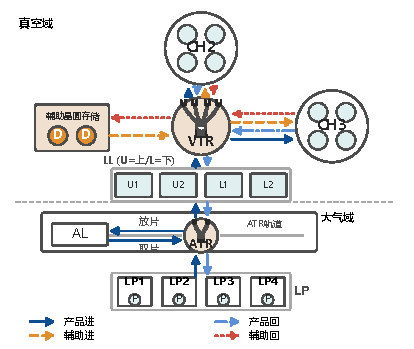
\includegraphics[width=0.72\linewidth]{fig_system_pjob_cn}
\caption{双源混流旋转腔组合设备拓扑与晶圆加工路径}\label{fig:system-zh-new}
\end{figure}

本文采用标称工艺参数构造算例，以分析晶圆组织与资源时序对排程的影响。调度对象为给定任务、设备参数和资源容量下的有限批次离线排程。
\section{研究内容与评价目标}
围绕有限计算时间内的排程质量，本文已开展的研究包括以下三个相互衔接的方面：

\begin{enumerate}
\item 建立以PW对为最小单元的两阶段MILP模型。按任务和来源LP统计产品数量，联合确定晶圆配对、腔室分配、加工周期、清洁和辅助片借还。第一阶段最小化批次完工时间，第二阶段保持该完工上界和主要离散决策，优化等待与节拍。
\item 设计结合结构化初始化与学习选割的RL-DMCT。先确定配对、分腔和加工周期，再逐层放开资源次序。根据候选割的变量角色特征进行学习排序，并按角色覆盖和候选相似度重排割子集。
\item 提出基于配对等待下界的双目标邻域搜索。由配对方式推导路线等待下界，结合指标上限筛选候选，对关联的配对、取放与设备次序联合调整，给出可按交期或等待要求选择的非支配排程。
\end{enumerate}


评价分别考察模型能否恢复满足设备约束的逐片排程、结构化初始解能否降低限时可行上界，以及共享初始解后学习选割能否带来额外改善。清洁规则、加工模式与辅助库存的对照用于解释排程的变化，阶段内对照用于分析等待与节拍。双目标实验还比较同预算下各方法的超体积，用两片算例的认证前沿检验覆盖度，并用两种75片配方组合复验逐片排程，检验相同初始结构与评价预算下局部调整生产块的收益。
\section{论文结构}
第一章说明研究背景、研究内容和评价目标。第二章梳理组合设备调度、时序约束与学习选割研究。第三章建立PW对联合模型并定义完工时间优先的两阶段目标。第四章介绍结构化初始解、变量角色特征与候选割重排，以及排程精修和解码流程，进而给出以配对等待下界筛选邻域的双目标搜索方法。第五章分析已完成的模型、初始化、选割、清洁与库存实验，展示2片最优排程和16片可行排程，比较两片认证前沿与75片混合批次的经验前沿。第六章归纳已有研究结论与后续方向。

\chapter{国内外研究现状}

组合设备（cluster tool，CT）调度研究起初关心连续加工同一类晶圆时，设备每隔多久能够产出一片晶圆。随着同一批次内出现多种工艺路线、一个腔室容纳多片晶圆，或者加工中途需要清洁腔室，决定产出的资源也会随设备状态而改变。对本文研究的旋转腔设备，有限批次的交付还取决于产品片、补位用的辅助片和清洁操作如何共用机械手，以及最后一片产品何时回到装载端口。下面沿着设备调度问题和求解方法两条线索梳理国内外研究。

\section{稳态吞吐率与驻留约束下的可调度性}

早期吞吐率模型把晶圆在腔室中接受工艺处理的时间与机械手搬运晶圆的时间放到同一周期内考察。1994年，Perkinson等分别计算单片和整批晶圆的加工时间，分析了工艺处理时间、搬运时间与设备最大吞吐率之间的关系\citep{perkinson1994throughput}。在机械手有充分时间服务各腔室时，缩短瓶颈工序的处理时间可以提高产出。当机械手已连续执行取放和移动动作时，即使增加腔室处理能力，晶圆仍需等候搬运。这使设备能力评价从单个腔室的标称加工时间转向腔室与机械手共同形成的周期。

晶圆加工结束后还可能受到残余气体或温度的影响，设备需要在工艺允许的时间窗内将其取出。于是，达到给定吞吐率的动作序列还要通过可调度性检验，即能否为该序列安排一组同时满足资源互斥和驻留上限的动作时刻。2002年，Rostami和Hamidzadeh同时考虑工艺模块与搬运模块的驻留限制，研究时间窗对设备调度的影响\citep{rostami2002optimal}。2010年，伍乃骐和周孟初针对双臂组合设备的稳态运行，从机械手等待时间推导可调度条件及最优稳态调度的闭式解\citep{wu2010closedform}。由此可以先判断重复动作序列能否在时限内执行，再计算可行序列所能达到的周期长度。

晶圆重入同一模块时，当前加工还要为同片晶圆后续再次访问该模块留下时间。2014年，乔岩等研究了原子层沉积中带重入和驻留约束的双臂组合设备，分析重复访问对机械手调度的影响\citep{qiao2014revisiting}。次年，乔岩在广东工业大学完成了关于半导体组合设备建模、优化调度与控制的博士论文\citep{qiao2015thesis}。对于更一般的离散事件系统，周家忠在西安电子科技大学的博士论文中采用时间扩展可达图表示操作顺序和时刻，通过集束搜索或状态聚类缩小搜索范围\citep{zhou2022thesis}。前一类工作利用特定设备结构推导时序性质，后一类方法则为动作顺序尚待搜索的情形提供了状态空间表示。袁凤连等在《自动化学报》的综述中归纳了这条研究脉络，并将驻留限制、作业时间波动、重入、多品种、模块故障、清洗和组合设备群列为七类典型问题\citep{yuan2023survey}。

\section{多品种投放、有限批次与多工位腔室}

从单一配方扩展到多品种后，即使各品种单独运行时都满足驻留上限，混合投放后仍要重新安排机械手。王际鹏等在2020年针对双臂组合设备提出多路交换序列，给出多种晶圆流模式下周期运行的可调度条件\citep{wang2020multiple}。当设备同时接收两类晶圆时，投放顺序还会改变并行腔室的负载。即使两种投放方案在一个周期内送入相同数量的晶圆，长工时晶圆集中到同一腔室，也会使另一腔室先完成加工并等待机械手。韩国研究者Ko等利用赋时事件图分析双臂设备，在保持最小周期时间的条件下，通过调整多类晶圆的投放顺序均衡并行腔室的负载，减少加工后的腔内等待\citep{ko2021balance}。2025年，Yang等将两类晶圆的投放顺序和单臂机械手的任务顺序同时作为混合整数规划的决策，分别评价周期吞吐率与驻留时间约束满足率\citep{yang2025miptwowafers}。因此，投放次序既决定哪一种产品先接受加工，也决定机械手随后需要优先服务哪一个腔室。

小批量生产中，设备尚未进入稳态，一个批次便可能接近结束。周期模型省去的首片入腔和末片离腔过程，此时会占据相当一部分批次时间。李金成和潘春荣研究单臂设备插入紧急订单后的暂态过程，针对不同加工参数推导插单可行条件及机械手等待时间\citep{li2023urgent}。罗亚波等进一步研究双臂设备的终止暂态，利用仍在加工末批晶圆的时间完成部分换模操作，在满足驻留约束的前提下缩短了算例中的换批时间\citep{luo2026mask}。从完整批次出发，Yang等也已针对两类晶圆建立单臂设备非周期调度模型，覆盖启动至收尾过程\citep{yang2025noncyclic}。因此，描述有限批次时，工艺路线之外还应明确完工事件取在末片离腔、完成后续搬运，还是回到原装载端口。

设备结构的扩展沿着不同的方向发展。多个并行腔室分别接收晶圆时，主要决策是如何分配负载。两个组合设备通过缓冲模块连接时，还要协调两台机械手对交接位置的访问。Kim在2023年的博士论文中用赋时事件图分析串联组合设备，再将反馈弧引入多周期序列的分析，以识别中间缓冲位置的阻塞及其造成的晶圆延迟\citep{kim2023tandemphd}。潘春荣等针对带全并行加工模块的双组合设备，利用面向资源的Petri网分析机械手任务冲突，给出了相应的可调度条件和稳态周期求解方法\citep{pan2024twin}。

将多个工位设在同一工艺腔内，又会引入不同的取片问题。Jee在韩国科学技术院完成的博士论文研究多槽位设备，考察一次处理多片晶圆后各片等待机械手取出的时间，并将多臂机械手的动作次序和含腔室清洁的设备配置纳入分析\citep{jee2021thesis}。Zou等研究有驻留时间约束的双工位单臂组合设备，进一步将同一模块内的多个工位纳入调度\citep{zou2024twospace}。

前端供片也会改变真空侧的可行时序。Huang等研究由设备前端、装载锁和真空模块组成的单臂设备，将前端搬运与真空侧时序放在同一设备内求解，并要求晶圆满足工艺驻留上限\citep{huang2025efem}。本文研究的双源分别供应产品晶圆和辅助晶圆。双源配置下，产品片从大气侧经装载锁进入真空侧，辅助片从真空存储区取用。产品品种决定加工需求，晶圆来源决定它占用的运输路径。两片晶圆即使能参加同一次加工，也必须能在同一装片窗口到达旋转腔的可访问工位。

\section{腔室清洁与辅助晶圆的复用}

安排清洁时，首先要区分清洁何时触发，以及触发后其他腔室如何继续生产。Yu和Lee研究双臂设备的腔室清洁，分析清洁周期内的晶圆延迟，通过减少向并行腔室装入的片数和调整机械手动作开始时刻控制等待\citep{yu2020delay}。乔岩等在双臂设备的周期序列中插入虚拟晶圆，使相应腔室能在该时段进行清洁，再用二元整数规划优化吞吐率\citep{qiao2022binary}。镇璐等在《系统工程理论与实践》讨论清洁时间较长的情形，为单臂设备设计两种机械手调度策略，并按工序分配等待时间以满足驻留限制\citep{zhen2023cnclean}。

对于按腔室状态触发的清洁，Li等研究了单臂设备的调度，Zhen等进一步处理双臂设备，给出在不同清洁情形下满足驻留约束并恢复稳态运行的策略\citep{li2022conditioncleaning,zhen2025cleaning}。多品种与清洁也已有联合研究，Yang等在两类晶圆、驻留限制及清洁并存的单臂设备上联合决定投放与机械手任务次序\citep{yang2025twoclean}。能否利用一段空闲时间清洁腔室，取决于清洁持续多久，也取决于这段时间内其他产品是否已到必须卸片的时刻。

在这些时序模型中，虚拟晶圆可以用来保留机械手动作序列中的位置。例如，罗亚波等用虚拟晶圆描述终止暂态中的换模时机\citep{luo2026mask}。制造现场的控片和挡片则有实物库存。Chen和Lee研究晶圆厂控片与挡片的补充、降级和回用，说明循环使用的非产品片同样需要库存控制\citep{chen2003dummy}。杨懿淑在新竹交通大学完成的博士论文进一步考虑多期需求的不确定性，通过随机规划确定新片供给和降级数量，并用服务水平约束控制缺片风险\citep{yang2009dummyphd}。这些工作回答了晶圆厂应准备多少片、怎样补充的问题。在设备调度中，还需知道已经借出的某一片何时能再次使用。

在本文的满片加工条件下，产品片数量不足时由辅助片占据空余工位，清洁时全部工位都要装入辅助片。于是，生产末端的补位会影响下一次清洁最早何时可以装片。即使两座腔室均已空闲，如果可用辅助片只够其中一座执行满片清洁，两次装片也要错开。描述这一约束需要把每片辅助片的源端取片、腔内占用和归还时刻连接起来。晶圆厂级的库存数量给出总量边界，设备动作序列给出每一时刻实际可借用的数量。

\section{驻留时间、路线等待与批内节拍}

调度方案的时间特性取决于测量的起止事件。缩短晶圆从加工结束到卸片的间隔，直接服务于驻留要求。在单周期产量相同的条件下，缩短平均开工间隔可以提高产出率，而缩小相邻间隔的差异则能使连续生产中的供片与取片更有规律。这几个指标可以在同一调度方案中呈现不同变化。朱清华等在双臂组合设备群上研究加工后停留时间，在取得最高吞吐率的同时优化工序加工后的总停留时间，并进一步用线性规划平衡相邻设备的停留时间差异\citep{zhu2023regulation}。2026年，Kim和Yu进一步以单片晶圆流经整台设备的时间为指标，研究调节设备内在制晶圆数的效果。在他们分析的设备中，降低装载水平可缩短单片流动时间，同时可能延长设备周期\citep{kim2026flow}。这两类结果说明，逐片时间可以在吞吐率相同的条件下得到改善，也可能需要以一部分产出为代价，具体取决于可以调整哪一类决策。

该区分在动作时间发生波动时尤其重要。Kim等研究随机时间扰动下的设备反馈控制，分析了设备受扰后晶圆停留时间能够重新稳定的条件\citep{kim2022feedback}。潘春荣等则在给定加工时间概率分布的条件下研究带并行腔室和周期清洁的设备，给出单臂设备平均周期时间的计算方法和双臂设备相应指标的近似算法\citep{pan2024variation}。前者处理执行中已经发生的偏差，后者预测许多周期的平均表现。本文给定各动作的标称时长，考察同一有限批次中由资源竞争造成的等待和间隔变化。

具体而言，本文以最后一片产品回到原装载端口的时刻衡量批次完工。对已经取得的可行排程，先保留其完工时间上界和主要离散决策，再调整连续时刻与允许变化的取放同步选择。路线等待扣除必要搬运或操作时长，分别统计总量和最大单项。链内节拍比较同一腔室、同一条$2\times2$加工链内连续三个生产周期形成的前后两个开始间隔。这样，同一份排程即可分别说明交付时刻、途中等待和链内节拍，清洁前后的间隔也不会混入同一条链的节拍评价。第三章式~\eqref{eq:primary-objective-cn}和式~\eqref{eq:secondary-rhythm-cn}给出了相应的计量边界。

\section{设备动作学习与混合整数规划选割}

组合设备中的强化学习首先可以作用于机械手。Kim和Lee研究两种晶圆在单臂设备上的并发加工，以强化学习和自适应搜索同时安排投放次序与机械手任务，使策略可以在预设周期序列之外选择动作\citep{kim2025adaptivecluster}。Kim和Kim针对非周期组合设备调度，将晶圆配方信息用于动作决策，结合当前调度状态选择下一步机械手动作以避免死锁\citep{kim2025noncyclicdeadlock}。2026年，Lai等进一步研究带设备前端的单臂设备，在由装载锁连接的大气侧和真空侧上开展非周期调度\citep{lai2026front}。在这些方法中，策略的一次选择会改变下一步哪些晶圆可以移动、哪些资源可供使用。

另一条路线先将设备约束写成混合整数线性规划（MILP），在分支定界搜索中用学习方法选择割平面。有效割可以排除线性松弛中的部分分数解，同时保留原整数可行解。Huang等将候选割选择表述为排序问题，利用多实例学习从候选割特征中估计优先级\citep{huang2022cutranking}。Paulus等以前瞻计算得到的界改善作为监督信号，用模仿学习近似开销较高的选割准则\citep{paulus2022looking}。两者处理的都是求解器已经生成的候选割，评价所选割时需要考虑松弛界改善及其计算代价。

Wang等在2023年的层次序列模型（HEM）中用上层策略确定选割数量，再用下层策略依次选出相应数量的割。2024年的期刊扩展研究了序列和集合两种候选表示，以及已选割之间的相互影响\citep{wang2023hem,wang2024hemset}。这一进展与旋转腔调度的联系在于，两个单独评分较高的割可能都集中在同一组腔室分配变量上，而候选集中还有涉及库存或机械手先后次序的割。第四章在HEM基础上提取变量角色特征并重排候选割。此处策略的输出是求解器采用的割集合与顺序，逐片排程仍从满足设备约束的整数可行解中解码。

\section{可行排程构造与原始解的邻域改进}

对最小化产品完工时间的模型，每一份完整可行排程都给出一个上界。寻找首个可行排程与改进已有排程可以利用不同的信息。前者可以从最难安排的资源入手。周炳海和黎明研究带并行腔的双集束型设备，围绕产能约束资源组织启发式调度，在多品种和驻留限制下协调并行腔与机械手\citep{zhou2016ccr}。对后者，已有排程还指明了具体的资源使用次序。例如，最后回片的产品若在装载锁前等待，缩短另一腔室一项与该产品无资源关联的动作，对其回片时刻没有影响。要使该产品提前回片，可能需要挪动此前占用同一装载锁或机械手的另一片晶圆。

通用整数规划为保留可行排程的大部分结构提供了两类邻域。2003年，Fischetti和Lodi提出局部分支，在当前整数解附近限制二元变量允许翻转的数量，由求解器在该范围内寻找改进解\citep{fischetti2003local}。Danna等提出松弛诱导邻域搜索（RINS），固定当前整数可行解与线性松弛解中取值一致的整数变量，再求解剩余子问题\citep{danna2005rins}。局部分支先限定改动幅度，RINS则依据两组解的一致性确定保留哪些决策。对具有实体库存的排程，移动一个产品对到另一腔室可能同时改变清洁触发位置、辅助片归还时刻和机械手次序。若邻域只允许改变分腔变量，相关动作就可能没有重新配合的余地。

邻域大小会影响子问题的求解成本。Hendel在SCIP中根据各大邻域启发式以往的收益选择下一个邻域，并通过固定变量调节子问题规模\citep{hendel2022alns}。Liu在蒙特利尔综合理工学院的博士论文中用学习方法确定局部分支的邻域大小，并利用优质解的结构特征选择变量生成邻域\citep{liu2022thesis}。对旋转腔设备，可进一步沿产品回片路径查找造成延迟的资源，联合放开有关的分配、占位与搬运次序，再用原MILP约束修复排程。可按相同计算预算下的可行上界和子问题耗时评价该邻域。本文的结构化初始化从配对、分腔和周期安排出发，为主问题建立初始上界。

\section{研究评述}

从稳态周期分析到多品种非周期调度，国内外研究已能在多种设备配置下联合确定投片和机械手动作，处理清洁、驻留及前端供片约束。控片与挡片的库存研究也已说明，可回用晶圆的供给会约束生产。对于本文的四工位旋转腔，这些问题在同一次换片中相遇。采用$4\times1$并行加工时，四个工位同批处理。采用$2\times2$链式加工时，一对晶圆要留在腔内继续处理，另一对要在旋转后换入或换出。模式选择因而同时决定哪一面可装卸、需要多少辅助片，以及两腔何时争用同一机械手。仅根据单腔的稳态周期或库存总量，无法还原这一动作序列。

表~\ref{tab:review-decisions}比较了与本文最接近的几项研究。是否将辅助片作为可返回的实体、是否记录每次取放，对问题的决策范围都有直接影响。

\begin{table}[htbp]
\centering
\caption{代表性研究的决策范围与评价对象}\label{tab:review-decisions}
\small
\begin{tabularx}{\textwidth}{@{}p{0.22\textwidth}XX@{}}
\toprule
研究 & 主要决策 & 评价对象 \\
\midrule
杨懿淑\citep{yang2009dummyphd} & 各期新片供给量、各等级控片与挡片的降级数量 & 不确定需求下的库存成本与服务水平 \\
Jee\citep{jee2021thesis} & 多槽位腔室的取放次序、机械手与腔室配置 & 同腔多片晶圆加工后的取片延迟 \\
镇璐等\citep{zhen2023cnclean} & 有清洁作业时各工序的机械手等待时间 & 驻留时限内的可行调度 \\
Yang等\citep{yang2025noncyclic} & 启动至收尾期间两类晶圆的投放和搬运顺序 & 有限批次的完成时间 \\
本文第三章 & 晶圆配对、分腔、旋转加工、辅助片借还与共享资源次序 & 最后产品回片时刻、路线等待与链内节拍 \\
\bottomrule
\end{tabularx}
\end{table}

第三章用晶圆对连接周期占位、辅助片借还与逐片路线。Sakai和Nishi已联合考察完工与腔内驻留时间\citep{sakai2017}。本文计量全路线等待与留片链节拍。第四章分别研究初始化、选割和基于配对等待下界的搜索，第五章在相同预算下比较上下界和前沿覆盖。

\chapter{基于PW对的两阶段调度模型}

\setcounter{equation}{0}

一次生产处理或清洁处理对应一个加工周期，其中生产周期指按产品配方执行工艺处理的周期。清洁处理仅由辅助晶圆占位，其阈值至少为2。

模型输入包括动作时长、资源容量、驻留上限、清洁阈值和辅助晶圆数量，输出为具体晶圆的资源指派及动作起止时刻。
表~\ref{tab:symbol-cn-a}定义输入常量与集合，表~\ref{tab:symbol-cn-b}定义主要决策变量及辅助变量，其余符号在正文首次使用处定义。
所有时刻和时长的单位均为秒，数量的单位为片、对或周期。

\begin{table}[!htbp]
\centering\small
\caption{批次任务调度的输入参数与集合配置}
\label{tab:symbol-cn-a}
\renewcommand{\arraystretch}{1.03}
\setlength{\tabcolsep}{4pt}
\begin{adjustbox}{max width=\linewidth,max totalheight=0.92\textheight}
\begin{tabular}{@{}>{\raggedright\arraybackslash}p{0.26\textwidth}p{\dimexpr0.74\textwidth-8pt\relax}@{}}
\toprule
符号 & 定义与取值\\\midrule
$\mathcal J,\mathrm{Pjob}_j$ & $\mathcal J=\{1,\ldots,J\}$是批次任务集合；$\mathrm{Pjob}_j$是任务$j$的产品晶圆集合。\\
$\mathcal L_j,\ell_{jk}$ & $\mathcal L_j$是任务$j$实际晶圆编号的升序表，$\ell_{jk}$是其第$k$片晶圆的来源LP编号。\\
$N_{j\ell},N_j,N_\zeta,N_\psi,N$ & 分别表示任务$j$在LP $\ell$的产品数、任务$j$的产品总数、两种生产配方的产品数及全批产品总数。\\
$m_j,\mathcal M,\mathcal C_j$ & $\mathcal M=\{\zeta,\psi,\mathrm{cl}\}$是加工类型集合，三种标签依次表示$4\times1$、$2\times2$与清洁；$m_j$是任务$j$的加工模式类型。$\mathcal C=\{\mathrm{CH2},\mathrm{CH3}\}$是腔室集合，$\mathcal C_j\subseteq\mathcal C$是任务$j$允许访问的非空腔室集合。\\
$\mathcal P,\mathcal Q_c,\mathcal I$ & $\mathcal P=\{1,\ldots,P_{\max}\}$是PW对集合；$\mathcal Q_c=\{1,\ldots,Q_{\max}\}$是腔室$c$的周期集合；$\mathcal I=\mathcal P\times\{0,1\}$是晶圆路线任务集合。\\
$T,J_{\max},P_{\max},Q_{\max}$ & 依次表示全设备生产周期数上界、清洁次数上界、PW对容量和每腔候选周期容量。\\
$\mathcal S,\sigma$ & $\mathcal S=\{A,V\}$是来源区域集合，元素分别是大气区、真空区；$\sigma$表示来源配置，单源取0、双源取1。\\
$\mathcal O,\mathcal O^{\rm occ}$ & $\mathcal O$是候选物理动作集合，$\mathcal O^{\rm occ}$是候选资源占用区间集合，由路线与周期模板生成。\\
$\mathcal R,K_\rho,\mathcal D$ & $\mathcal R$是资源集合，$K_\rho$是资源$\rho$的容量：ATR承2片、VTR承4片，AL容量1片，上/下LL各2槽，腔室4工位，$\mathcal D=\{1,\ldots,D\}$是辅助晶圆集合，默认$D=8$，两个腔时存储容量为10片。\\
$d_m\ (d_\zeta,d_\psi,d_{\mathrm{cl}})$ & 表示类型$m$的加工持续时间，默认$(d_\zeta,d_\psi,d_{\mathrm{cl}})=(180,90,500)$~s；$2\times2$产品需相邻两次加工处理。\\
$d_o^{\rm ATR},d_o^{\rm VTR},r_c$ & 分别表示ATR取放时长、VTR取放时长和腔室$c$半周旋转时长，默认分别为4、1、2~s。\\
$t_{\rm ATR},t_{\rm VTR},t_{\rm empty}$ & 分别表示ATR交换时长、VTR交换时长和ATR从LL移动LP的时长，默认分别为3、2、6~s。\\
$t_{\rm AL},t_{\rm pump},t_{\rm vent}$ & 分别表示产品对准、上LL抽气及下LL放气时长，默认分别为20、30、25~s；辅助片不执行AL对准。\\
$t_{\rm U}^{\rm reset},t_{\rm L}^{\rm reset}$ & 分别表示上/下LL槽位复位时长，默认分别为30、25~s，从另一侧取片结束后开始计。\\
$d_o,\delta_{oo'},\delta^\rho_{oo'}$ & 分别表示动作$o$的持续时间、$o$结束至后续动作$o'$开始的时间间隔、资源$\rho$从$o$至$o'$的换位或复位间隔。\\
$H$ & 表示清洁阈值，$H\ge2$，默认$H=3$；累计1至$H-1$次可提前清洁，达到$H$必须清洁。\\
$\overline R_{i\rho}$ & 表示路线任务$i$在资源$\rho$的驻留上限；模块按放片结束至取片开始计，工艺腔另扣除必要处理时长；机械手按取片开始至放片结束计。\\
$B,M$ & 分别表示整个加工排程的时间上界和加上必要间隔的约束松弛量；默认$B=10000$~s，装载锁复位须在时域内完成；后者取$M=B+\max\{\delta_{oo'},\delta^\rho_{oo'},r_c\}$。\\
$\lambda_1,\lambda_2,\lambda_3$ & 依次是总等待、最大单项等待与节拍变化的非负权重，默认$(\lambda_1,\lambda_2,\lambda_3)=(1,10,25)$。\\
$\varepsilon_C$ & 产品完工上界容差，默认$10^{-6}$~s。\\
\bottomrule
\end{tabular}
\end{adjustbox}
\end{table}

\begin{table}[!htbp]
\centering\small
\caption{批次任务调度的关键决策变量}
\label{tab:symbol-cn-b}
\renewcommand{\arraystretch}{1.05}
\setlength{\tabcolsep}{4pt}
\begin{adjustbox}{max width=\linewidth}
\begin{tabular}{@{}>{\raggedright\arraybackslash}p{0.23\textwidth}p{0.18\textwidth}p{0.55\textwidth}@{}}
\toprule
符号 & 类型 & 定义与取值含义\\\midrule
$x_{j\ell pr}$ & 二元决策变量 & PW对$p$的位置$r$是否使用任务$j$在LP $\ell$的一片产品，$N_{j\ell}>0$时建立。\\
$v_p,\mu_{pm},z_{pc}$ & 二元决策变量 & 分别表示PW对$p$是否启用，是否采用加工类型$m$，是否分配至腔室$c$。\\
$X_{pcq},K_{cqm},f_{pcq}$ & 二元决策变量 & 分别表示PW对$p$是否占用腔室$c$的周期$q$，周期$q$是否采用类型$m$，对$p$在腔室$c$的周期$q$是否位于可访问侧。\\
$g_{pr\tau}$ & 二元决策变量 & 表示对内位置$(p,r)$是否借用辅助晶圆$\tau\in\mathcal D$。\\
$h_{ou},y^\rho_{oo'},\gamma_{pa}$ & 二元决策变量 & 分别表示动作$o$是否选择物理单元$u$，在同一资源$\rho$时$o$是否先于$o'$，对$p$的两片晶圆在取放段$a$同步搬运，标签$\mathrm{pick}$表示源LP端取片。\\
$s_o,S_{cq}$ & 非负实数决策变量 & 分别表示物理动作$o$和腔室$c$的周期$q$的开始时刻。\\
$e_o,b_o$ & 辅助变量 & $e_o$表示动作$o$的结束时刻；$b_o$是二元辅助变量，表示动作$o$是否启用。\\
$\theta_{j\ell}$ & 非负实数辅助变量 & 任务$j$在相邻非空LP之间切换取片的时间分界点。\\
$n_{cq}$ & 非负整数辅助变量 & 腔室$c$第$q$个周期结束后，自上次清洁以来累计完成的生产周期数，范围为$0,\ldots,H$。\\
$F_p,F_p^\psi,X^P_{pcq}$ & 二元辅助变量 & 分别表示对$p$是否含产品，是否含$2\times2$产品，是否参加腔室$c$的周期$q$。\\
$\beta_{pr},d_{pr}$ & 二元辅助变量 & $\beta_{pr},d_{pr}$ 分别表示对内位置$(p,r)$是否安排产品、是否借用辅助片。\\
$\chi_{iA},\chi_{iV}$ & 二元辅助变量 & $\chi_{iA},\chi_{iV}$分别表示路线任务$i$是否由大气区、真空区供给。\\
$C_{\max}$ & 非负实数决策变量 & 产品返回原LP时刻的上界。\\
$L_{\max},v_{cq}$ & 非负实数辅助变量 & $L_{\max}$为所有等待项的上界；$v_{cq}$为以$(c,q)$为中心的相邻周期开始间隔变化量的绝对值上界。\\
\bottomrule
\end{tabular}
\end{adjustbox}
\end{table}

\section{批次任务与产品晶圆编码}
\label{sec:model-encoding-cn}

产品晶圆按工艺模式、可访问腔室及其他调度属性分组，每片恰属于一个批次任务。同任务、同LP的产品须具有相同调度属性，才能以库存数量表示；若释放时刻、工艺要求或槽位可访问性不同，应细分任务或显式增加区分约束。允许腔室集合可为$\{\mathrm{CH2}\}$、$\{\mathrm{CH3}\}$或$\{\mathrm{CH2},\mathrm{CH3}\}$。

输入编码依次完成实际编号、任务内排序和编号映射。$w$表示输入产品晶圆的实际编号，由其LP
与槽位计算：$w=25(\ell-1)+s$。$\mathcal L_j[k]$表示有序表$\mathcal L_j$的第$k$项，
$\mathrm{Pjob}_j[k]$表示该项对应晶圆的批次内标识。$k_j(w)$是整数常量，表示晶圆$w$在
该表中的排序位置；$w'$是计数时遍历该表的实际编号索引。$\mathsf{Code}$是编号映射函数，
将实际编号转换为批次内标识：

\begin{equation}
\begin{aligned}
k_j(w)&=1+|\{w'\in\mathcal L_j:w'<w\}|,\\
\mathsf{Code}(w)&=\mathrm{Pjob}_j[k_j(w)],\\
\ell_{jk}&=1+\left\lfloor\frac{\mathcal L_j[k]-1}{25}\right\rfloor,
\quad k=1,\ldots,N_j.
\end{aligned}
\label{eq:pjob-input-code-cn}
\end{equation}

其中，$\mathsf{Code}^{-1}$是上述编号映射的逆函数，可通过$\mathsf{Code}^{-1}(\mathrm{Pjob}_j[k])=\mathcal L_j[k]$还原实际编号。
按来源LP计数可得$N_{j\ell}=|\{k:\ell_{jk}=\ell\}|$。批次内编号连续，实
际编号可因槽位空缺或属于其他任务而不连续。编码实例见表~\ref{tab:pjob-code-example-cn}。

\begin{table}[!htbp]
\centering\footnotesize
\caption{实际晶圆编号到批次内编号的映射示例}
\label{tab:pjob-code-example-cn}
\begin{adjustbox}{max width=\linewidth}
\begin{tabular}{cccc}
\toprule
实际编号$w$ & LP/槽位$(\ell,s)$ & 批次内序号$k$ & $\mathsf{Code}(w)$\\
\midrule
1 & $(1,1)$ & 1 & $\mathrm{Pjob}_1[1]$\\
3 & $(1,3)$ & 2 & $\mathrm{Pjob}_1[2]$\\
26 & $(2,1)$ & 3 & $\mathrm{Pjob}_1[3]$\\
27 & $(2,2)$ & 4 & $\mathrm{Pjob}_1[4]$\\
2 & $(1,2)$ & 1 & $\mathrm{Pjob}_2[1]$\\
\bottomrule
\end{tabular}
\end{adjustbox}
\end{table}

Pjob是同质产品的任务与库存组。模型以两片晶圆组成的PW对为最小单元安排腔室加工与成对搬运，一个满片周期同时处理两个PW对。每个PW对包含两个位置，分别记录晶圆来源、对准及供回片动作时刻。批次内出片顺序由第~\ref{sec:model-assignment-cn}节的指派与时间约束保证。

\section{单源与双源混流物理加工路径}
\label{sec:model-path-cn}

来源选择变量与晶圆类型及配置$\sigma$满足：

\begin{equation}
\begin{aligned}
\chi_{iA}&=\beta_{pr}+(1-\sigma)d_{pr},\\
\chi_{iV}&=\sigma d_{pr},\qquad i=(p,r)\in\mathcal I.
\end{aligned}
\label{eq:source-membership-cn}
\end{equation}

式~\eqref{eq:source-membership-cn}规定每个晶圆路线任务的来源区域。单源配置下，产品位于LP1--LP4，辅
助晶圆位于LP4旁的大气存储区，两者共享ATR和装载锁接口，但只有产品需要AL对准。双源配置下，产品晶圆仍来自
LP1--LP4，辅助晶圆则由真空区存储位供给。

产品路线采用图~\ref{fig:system-zh-new}所示的物理路径。

辅助晶圆不执行AL对准。单源辅助晶圆从LP4旁的大气存储区出发，经ATR、上装载锁和VTR进入工艺腔室，使用后经
VTR、下装载锁和ATR返回原存储区。单独供给时，辅助晶圆绕过AL直接入锁；随产品入片时，辅助晶圆在产品对准期
间保持在ATR上，待产品取回后共同入LL，见图~\ref{fig:single-source-cn}。双源辅助晶圆从真空存储区出发，
经VTR进入工艺腔室，使用后由VTR返回真空存储区。上述路径确定晶圆必须经历的物理环节，成对搬运选择及其时间
条件在第~\ref{sec:model-time-cn}节给出。

\begin{figure}[!htbp]
\centering
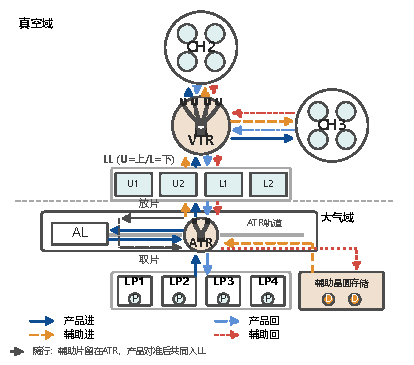
\includegraphics[width=\linewidth]{fig_single_source_pjob_cn}
\caption{单源旋转腔组合设备的拓扑与晶圆路线。}
\label{fig:single-source-cn}
\end{figure}

\section{晶圆、PW对与腔室周期的匹配关系}
\label{sec:model-assignment-cn}

$4\times1$模式在相邻加工周期之间更换全部4片晶圆，$2\times2$模式每次更换2片晶圆并保留另2片继续处理。因此，
将晶圆组织为PW对，再将PW对分配到兼容腔室及其加工周期。每个PW对包含两片晶圆，对内位置$r\in\{0,1\}$是配对索引，
实际承片位置和腔内占位由后续资源与周期变量确定。生产与清洁共用候选加工周期，具体生产次数和清洁规则见第~\ref{sec:model-process-cn}节。

\noindent\textbf{晶圆配对与腔室选择：}
一个PW对可由两片产品、一片产品与一片辅助晶圆，或两片辅助晶圆组成。所有产品均须安排加工，且每个启用对内位置恰好安排一片晶圆。因此，有
\begin{equation}
\begin{aligned}
\sum_{p,r}x_{j\ell pr}&=N_{j\ell},\\
\beta_{pr}=\sum_{j,\ell}x_{j\ell pr},\qquad
\beta_{pr}+d_{pr}&=v_p.
\end{aligned}
\label{eq:joint-membership-cn}
\end{equation}
式~\eqref{eq:joint-membership-cn}满足各任务的LP库存与对内位置唯一占用要求；各位置保留完整加工路线，实际产品身份在求解后恢复。
动作下标$o$可写成$(i,a)$、$(p,a)$或$(c,q,a)$，分别定位晶圆路线、PW对或腔室周期中的动作，$a$为动作标签；起止时刻统一记为$s_o,e_o$。

\noindent\textbf{批次内非递减顺序出片：}
按给定的非递减出片规则，同一批次任务在较小编号LP中的产品取片不得晚于下一非空LP中的产品。
$h_j(\ell)=\min\{\ell'>\ell:N_{j\ell'}>0\}$表示任务$j$在LP $\ell$之后的首个非空LP编号，集合为空时不
建立对应变量。对每个对内位置$(p,r)$，以下$o=((p,r),\mathrm{pick})$定位其LP取片动作。相邻非空LP之间满足：
\begin{equation}
\begin{aligned}
0\le\theta_{j\ell}&\le B,\\
s_o&\le\theta_{j\ell}+M(1-x_{j\ell pr}),\\
s_o&\ge\theta_{j\ell}-M(1-x_{j,h_j(\ell),pr}).
\end{aligned}
\label{eq:pjob-release-boundary-cn}
\end{equation}
式~\eqref{eq:pjob-release-boundary-cn}约束跨LP取片顺序，同一任务、同一LP的产品按取片时刻恢复实际编号，从而满足批次内非递减出片。同一PW对中来自同一LP的产品允许同步取片，但仍须满足式~\eqref{eq:stage-link-cn}及机械手容量约束；其他取片按ATR互斥与换位条件执行。不同Pjob可交错取片，并在工艺相容时组对。

同一PW对中的两片晶圆应采用相容的工艺模式，并进入共同允许的腔室。令$\mathcal C(m)\subseteq\mathcal C$为可执行加工类型$m$的腔室集合，模式与腔室选择满足：
\begin{equation}
\begin{aligned}
\sum_m\mu_{pm}&=v_p,\qquad \sum_c z_{pc}=v_p,\\
x_{j\ell pr}&\le\mu_{p,m_j},\qquad
x_{j\ell pr}\le\sum_{c\in\mathcal C_j}z_{pc},\\
z_{pc}+\mu_{pm}&\le1\qquad(c\notin\mathcal C(m)).
\end{aligned}
\label{eq:joint-chamber-cn}
\end{equation}
同模式的不同任务可组对，所选腔室须属于对内产品允许腔室集合的交集；允许访问两腔的任务可将不同PW对分配至不同腔室。

产品状态、链式模式标记与清洁类型之间满足：
\begin{equation}
\begin{aligned}
F_p&\le\sum_r\beta_{pr}\le2F_p,\qquad F_p+\mu_{p,\mathrm{cl}}\le1,\\
F_p^\psi&\le F_p,\quad F_p^\psi\le\mu_{p\psi},\quad
F_p^\psi\ge F_p+\mu_{p\psi}-1.
\end{aligned}
\label{eq:pair-type-cn}
\end{equation}
位置$(p,r)$的产品来源及回片LP直接由$\sum_jx_{j\ell pr}$确定，辅助来源位置分别由$(1-\sigma)d_{pr}$与$\sigma d_{pr}$确定。

\noindent\textbf{候选容量上界：}
为联合配对与周期决策预留足够的候选编号，采用以下保守容量上界：
\begin{equation}
\begin{gathered}
T=N_{\zeta}+2N_{\psi},\qquad J_{\max}=T,\\
P_{\max}=N+T+2J_{\max},\qquad Q_{\max}=T+J_{\max}.
\end{gathered}
\label{eq:candidate-bounds-cn}
\end{equation}
每个生产周期至少含一片产品，故生产周期数不超过总处理次数$T$；每次清洁前至少有一个生产周期，故清洁次数不超过$T$。含产品对、生产补位对和清洁对分别至多为$N$、$T$和$2J_{\max}$个，得到式~\eqref{eq:candidate-bounds-cn}的容量上界，保留所有合法的提前清洁选择。PW对按一次装入至卸出的占位任务编号，与可复用实体辅助片的库存分别计量。

\noindent\textbf{PW对与加工周期匹配：}
腔室执行生产或清洁时均应保持四工位满片，即每个周期恰好容纳两个PW对。$U_{cq}$是二元辅助变量，表示腔室$c$的周期$q$是否启用。所选
PW对的腔室与加工类型须与周期一致，因此，有：
\begin{equation}
\begin{aligned}
\sum_mK_{cqm}&=U_{cq}, &\sum_pX_{pcq}&=2U_{cq},\\
X_{pcq}&\le z_{pc}, &X_{pcq}+\mu_{pm}&\le1+K_{cqm},\\
\sum_pX^P_{pcq}&\ge K_{cq\zeta}+K_{cq\psi}, &U_{c,q+1}&\le U_{cq},\\
\sum_{c,q}U_{cq}&\le Q_{\max}, &\sum_{c,q}K_{cq,\mathrm{cl}}&\le J_{\max}.
\end{aligned}
\label{eq:cycle-capacity-cn}
\end{equation}
含产品PW对是否参与加工周期，由以下线性约束确定：
\begin{equation}
X^P_{pcq}\le X_{pcq},\quad X^P_{pcq}\le F_p,\quad
X^P_{pcq}\ge X_{pcq}+F_p-1.
\label{eq:cycle-products-cn}
\end{equation}
式~\eqref{eq:cycle-capacity-cn}保证满片加工、PW对与周期相容及候选容量限制；式~\eqref{eq:cycle-products-cn}保证只有含产品对的
占位计入生产要求。由此，生产周期至少含一个产品对，清洁周期只含辅助对。周期按编号连续启用，但不同加工模式的先后次序仍由模型确定。

\section{动作时间与先后逻辑}
\label{sec:model-time-cn}

晶圆操作须满足路线先后关系，成对搬运还须满足两片晶圆的取放同步条件；共享资源的服务次序由第~\ref{sec:model-resource-cn}节的约束确定。

\noindent\textbf{动作启用与持续时间：}
动作启用状态由所选晶圆路线、腔室周期及搬运方式共同确定。已启用动作的持续时间为输入参数，未启用动作的起止时刻均置零；其中LP取片时长满足$d_o>0$。因此，有：
\begin{equation}
0\le s_o\le B b_o,\qquad
0\le e_o\le B b_o,\qquad
e_o=s_o+d_ob_o.
\label{eq:operation-time-cn}
\end{equation}
式~\eqref{eq:operation-time-cn}保证取放、对准、压力转换、旋转及加工动作按给定时长执行，等待只能发生在动作之间。产品对准动作由$\beta_{pr}$启用，源端、ATR与装载锁动作由$\beta_{pr}+(1-\sigma)d_{pr}$启用，VTR供回动作由$v_p$启用。

\noindent\textbf{路径对应的动作先后关系：}
令$\mathcal A$为腔内共同动作链与各晶圆供回路线的已启用先后弧集合；供回路线按来源$\chi_{i\varsigma}$及成对搬运、单源随行入片选择启用，$\varsigma\in\mathcal S$。对弧$(o,o')\in\mathcal A$，后继须在前驱完成并经过必要间隔后开始，且后继启用时前驱也须启用：
\begin{equation}
b_{o'}\le b_o,\qquad
s_{o'}\ge e_o+\delta_{oo'}-M(2-b_o-b_{o'}).
\label{eq:precedence-cn}
\end{equation}
式~\eqref{eq:precedence-cn}连接所选路线的装载、加工与卸载事件。时刻均在$[0,B]$内，$M$覆盖时域与必要间隔，使未启用条件下的时序约束充分放松。

\noindent\textbf{单片、批次与成对搬运动作的同步：}
对需同步的动作$o,o'$，令$x$引用相应LP所属、周期占位或搬运选择的既有二元变量，统一要求：
\begin{equation}
\begin{aligned}
-M(1-x)&\le s_o-s_{o'}\le M(1-x),\\
-M(1-x)&\le e_o-e_{o'}\le M(1-x).
\end{aligned}
\label{eq:stage-link-cn}
\end{equation}
式~\eqref{eq:stage-link-cn}使单片动作与其所属批次的对应动作同时开始、同时结束；成对搬运取$x=\gamma_{pa}$、$o=((p,0),a)$及$o'=((p,1),a)$。同步时机械手执行一次共同动作，与其他动作保持互斥，两片晶圆仍分别占用承片位置；未同步时按式~\eqref{eq:resource-order-cn}分别排序。

\noindent\textbf{单源产品--辅助对的入片逻辑：}
对于单源产品--辅助对，$i_{\rm P},i_{\rm D}$是路线任务索引，分别表示该对中产品与辅助晶圆的路线，下标$\mathrm P,\mathrm D$是晶圆类型标签。
$\gamma^{\rm early}_p,\gamma^{\rm late}_p,\gamma_{p,\mathrm{in}}$是二元决策变量，分别表示是否选择辅助晶圆先行入锁、产品放至AL后再取辅助
晶圆、辅助晶圆随产品入锁。动作标签$\mathrm{ALput,ALpick,LLput}$分别表示放至AL、从AL取回和放入上装载锁。三种路线择一：
\begin{equation}
\begin{gathered}
\gamma^{\rm early}_p+\gamma^{\rm late}_p+\gamma_{p,\mathrm{in}}=1,\\
\gamma^{\rm early}_p=1\Rightarrow e_{(i_{\rm D},\mathrm{LLput})}\le s_{(i_{\rm P},\mathrm{ALput})},\\
\gamma^{\rm late}_p=1\Rightarrow s_{(i_{\rm D},\mathrm{pick})}\ge e_{(i_{\rm P},\mathrm{ALput})},\\
\gamma_{p,\mathrm{in}}=1\ \Longrightarrow
\begin{cases}
e_{(i_{\rm D},\mathrm{pick})}\le s_{(i_{\rm P},\mathrm{ALput})},\\
s_{(i_{\rm D},\mathrm{LLput})}=s_{(i_{\rm P},\mathrm{LLput})},\\
e_{(i_{\rm D},\mathrm{LLput})}=e_{(i_{\rm P},\mathrm{LLput})},\\
s_{(i_{\rm P},\mathrm{LLput})}\ge e_{(i_{\rm P},\mathrm{ALpick})}.
\end{cases}\end{gathered}
\label{eq:single-source-accompany-cn}
\end{equation}
该条件表示辅助晶圆在产品放至AL前已由ATR承载，并与完成对准的产品同时放入上装载锁。辅助晶圆从源端取片至入锁结束持续占用一个ATR承片位置；产品占
用AL期间不占用ATR承片位置，取回后恢复占用。若辅助晶圆单独供给，则直接连接其源端取片与入锁事件。

\section{两种工艺模式与清洁处理}
\label{sec:model-process-cn}

在第~\ref{sec:model-assignment-cn}节的PW对与周期指派关系基础上，进一步约束加工次数、相邻周期的占位连续性、旋转装卸次序及清洁边界；时刻变量沿用第~\ref{sec:model-time-cn}节的定义。

\noindent\textbf{生产模式与连续占位：}
图~\ref{fig:chain-zh}和图~\ref{fig:parallel-zh}给出两种工艺模式的事件顺序，其加工次数与连续性由周期占位约束描述。

\begin{figure}[t]
\centering
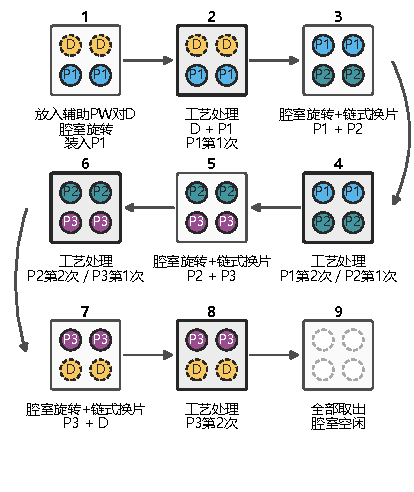
\includegraphics[width=0.93\linewidth]{fig_chain_cn_nature}
\caption{$2\times2$链式生产的事件顺序，D表示辅助PW对。}
\label{fig:chain-zh}
\end{figure}

\begin{figure}[t]
\centering
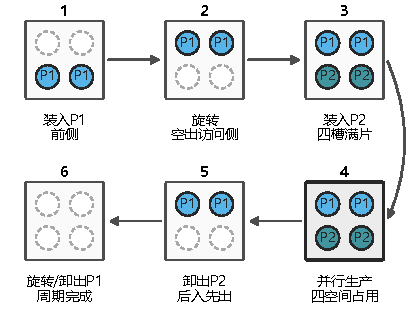
\includegraphics[width=\linewidth]{fig_parallel_cn_nature}
\caption{$4\times1$并行生产的事件顺序。}
\label{fig:parallel-zh}
\end{figure}

$A_{pcq},Z_{pcq}$是二元辅助变量，分别表示对$p$是否在腔室$c$的周期$q$首次、末次参加处理；$A^\psi_{pcq},Z^\psi_{pcq}$是二元辅助变量，分别表示上
述首次、末次参加处理的对是否为$2\times2$含产品对。取边界$X_{pc0}=X_{pc,Q_{\max}+1}=A_{pc,Q_{\max}+1}=0$，且$A_{pc1}=X_{pc1}$直接代入，有：
\begin{equation}
\begin{aligned}
A_{pcq}&\ge X_{pcq}-X_{pc,q-1}, &A_{pcq}&\le X_{pcq},\\
A_{pcq}&\le1-X_{pc,q-1},\\
Z_{pcq}&=X_{pcq}-X_{pc,q+1}+A_{pc,q+1},\\
\sum_{c,q}X_{pcq}&=v_p+F_p^{\psi}, &\sum_{c,q}A_{pcq}&=v_p,\\
A^{\psi}_{pcq}&=X_{pcq}-Z_{pcq}, &Z^{\psi}_{pcq}&=X_{pcq}-A_{pcq},\\
\sum_pA^{\psi}_{pcq}&\le1, &\sum_pZ^{\psi}_{pcq}&\le1.
\end{aligned}
\label{eq:cycle-exposures-cn}
\end{equation}
式~\eqref{eq:cycle-exposures-cn}使每个启用PW对只进入腔室一次，并连续参加一个或两个周期。前三条不等式给出$A_{pcq}=X_{pcq}(1-X_{pc,q-1})$，结合末
次参加标记可得$\sum_{c,q}Z_{pcq}=\sum_{c,q}A_{pcq}=v_p$。含产品的$4\times1$对参加一次处理，含产品的$2\times2$对在同腔参加相邻两次处理，纯辅助补
位对与清洁对均只参加一个周期。

\noindent\textbf{加工时长与周期先后关系：}
一个加工周期只有在前一周期结束后才能开始，持续时间由所选加工类型确定，周期结束时刻为$S_{cq}+\sum_m d_mK_{cqm}$，因此，有
\begin{equation}
\begin{aligned}
S_{cq}&\ge0,\\
S_{cq}+\sum_m d_mK_{cqm}&\le B U_{cq},\\
S_{cq}&\ge S_{c,q-1}+\sum_m d_mK_{c,q-1,m}\\
&\quad-M(1-U_{cq})\qquad(q>1).
\end{aligned}
\label{eq:cycle-time-cn}
\end{equation}
该约束固定各类加工周期的持续时间，等待仅发生在动作之间；装卸与旋转的持续时间由相应事件单独计入。

\noindent\textbf{前后侧占位与旋转装卸：}
机械手只能访问腔室前侧，故新装入的PW对位于前侧，保留自上一周期的PW对经旋转转至后侧。$\kappa_{cq},\upsilon_{cq}$是二元辅助变量，分别表示周期$q$是否保
留来自$q-1$的一个PW对、周期$q$结束后是否两个PW对全部退出。根据相邻周期的占位关系，有
\begin{equation}
\begin{aligned}
\kappa_{cq}&=\sum_p(X_{pcq}-A_{pcq}),\\
\upsilon_{cq}&=U_{cq}-\sum_p(X_{pcq}-Z_{pcq}),\\
f_{pcq}&\le A_{pcq},\qquad\sum_pf_{pcq}=U_{cq},\\
f_{pc,q-1}&\ge X_{pcq}-A_{pcq}\quad(q>1),\\
f_{pcq}&\ge F_p+K_{cq\psi}+X_{pcq}-2-\kappa_{cq}.
\end{aligned}
\label{eq:cycle-side-cn}
\end{equation}
动作$(p,\mathrm{load})$与$(p,\mathrm{unload})$分别是PW对$p$的装入与卸出；$(c,q,\mathrm{rot-})$与$(c,q,\mathrm{rot+})$分别是该周期前、后的半周旋转，
由$U_{cq}$与$\upsilon_{cq}$启用，各持续$r_c$，装入与旋转的时序约束为
\begin{equation}
\begin{aligned}
X_{pcq}=1\ \Rightarrow\quad
&S_{cq}\ge e_{(p,\mathrm{load})},\\
&s_{(p,\mathrm{unload})}\ge S_{cq}+\sum_m d_mK_{cqm};\\
A_{pcq}=1,\ f_{pcq}=0\ \Rightarrow\quad
&e_{(p,\mathrm{load})}\le s_{(c,q,\mathrm{rot-})};\\
A_{pcq}=1,\ f_{pcq}=1\ \Rightarrow\quad
&s_{(p,\mathrm{load})}\ge e_{(c,q,\mathrm{rot-})},\\
&S_{cq}=e_{(p,\mathrm{load})};\\
\kappa_{cq}=1\ \Rightarrow\quad
&s_{(c,q,\mathrm{rot-})}\ge S_{c,q-1}\\
&\qquad+\sum_m d_mK_{c,q-1,m}.
\end{aligned}
\label{eq:cycle-load-cn}
\end{equation}
全部退出时，周期后旋转在加工结束后开始。最后一次加工后的卸片关系为
\begin{equation}
\begin{aligned}
Z_{pcq}=1,\ f_{pcq}=1\quad
&\Rightarrow e_{(p,\mathrm{unload})}\le s_{(c,q,\mathrm{rot+})},\\
Z_{pcq}=1,\ f_{pcq}=0,\ \upsilon_{cq}=1\quad
&\Rightarrow s_{(p,\mathrm{unload})}\ge e_{(c,q,\mathrm{rot+})},\\
Z_{pcq}=1,\ f_{pcq}=0,\ \upsilon_{cq}=0\quad
&\Rightarrow s_{(p,\mathrm{unload})}\ge e_{(c,q+1,\mathrm{rot-})}.
\end{aligned}
\label{eq:cycle-unload-cn}
\end{equation}
下一周期新装入的PW对必须等待上一周期所有退出对完成卸载。对$p,p'\in\mathcal P$及$q>1$，有：
\begin{equation}
\begin{aligned}
s_{(p',\mathrm{load})}&\ge e_{(p,\mathrm{unload})}\\
&\quad-M(2-Z_{pc,q-1}-A_{p'cq}).
\end{aligned}
\label{eq:cycle-exchange-cn}
\end{equation}
保留一个对时，式~\eqref{eq:cycle-exchange-cn}仅等待被替换对卸出；全部退出时则等待两对均卸完，并与VTR动作互斥共同约束换片。

\noindent\textbf{清洁触发与清洁动作链：}
用清洁计数器累计自上次清洁以来的生产周期数，完成清洁后计数归零。达到阈值时须执行清洁，未达到阈值时可在合法工艺边界提前清洁；初始清洁与连续清洁均不允许。
取候选尾部$U_{c,Q_{\max}+1}=0$，有：
\begin{equation}
\begin{aligned}
0\le n_{cq}&\le H U_{cq},\qquad n_{c0}=0,\\
K_{cq,\mathrm{cl}}=1&\Rightarrow n_{cq}=0,\\
U_{cq}=1,\ K_{cq,\mathrm{cl}}=0
&\Rightarrow n_{cq}=n_{c,q-1}+1,\quad n_{c,q-1}\le H-1,\\
K_{cq,\mathrm{cl}}=1&\Rightarrow 1\le n_{c,q-1}\le H,\\
n_{cq}&\le H-1+H U_{c,q+1}.
\end{aligned}
\label{eq:clean-counter-cn}
\end{equation}
式~\eqref{eq:clean-counter-cn}在达到阈值时强制清洁，包括最后一个生产段；初始计数为零、清洁前计数至少为1及清洁后归零共同禁止初始清洁和连续清洁。由式~\eqref{eq:cycle-capacity-cn}与式~\eqref{eq:cycle-exposures-cn}，同一链式产品对须连续参加两个生产周期，清洁不能插入其中。

清洁作为$m=\mathrm{cl}$的满片周期，由两个纯辅助PW对占位，与生产共用式~\eqref{eq:cycle-load-cn}--\eqref{eq:cycle-exchange-cn}的装卸与旋转规则：两侧装入四片辅助晶圆后清洁，再依次卸出。相邻周期的换片约束要求清洁前卸完原有晶圆，清洁后卸完辅助片，再装入下一周期的晶圆；VTR互斥及辅助片借还约束共同确定搬运与复用时刻。

\section{辅助晶圆复用与机械手、模块资源}
\label{sec:model-resource-cn}

实体资源可用性通过辅助晶圆身份指派、机械手承片位置与模块槽位分配、占用互斥及驻留上限约束共同保证。

\noindent\textbf{辅助晶圆与循环复用：}
两腔共享辅助晶圆库存，一片辅助晶圆在归还之前不能再次借出。因此，每项有效借用需求应选定一片实体晶圆，同一PW对的两个位置应使用不同晶圆，有
\begin{equation}
\sum_{\tau\in\mathcal D}g_{pr\tau}=d_{pr},\qquad
\sum_{r=0}^{1}g_{pr\tau}\le1.
\label{eq:dummy-assign-cn}
\end{equation}
式~\eqref{eq:dummy-assign-cn}保证每项辅助需求恰好分配一片晶圆。借用区间按共享资源约束排序，使同一晶圆只能在完成归还后再次使用。该条件同样适用于跨
腔借用，允许两腔使用不同辅助晶圆并行生产。

\noindent\textbf{机械手与模块容量：}
资源排序区分执行机构的动作互斥与承片位置的容量限制。ATR、VTR、AL及各旋转腔的执行机构作为独占动作资源；机械手承片位置、装载锁槽位和辅助晶圆身份分别分配物理单元，容量采用表~\ref{tab:symbol-cn-a}的配置。腔内占位已由式~\eqref{eq:cycle-capacity-cn}约束。

资源分配以单个占用区间为单位：一次单片承片位置占用、一次辅助晶圆借用或一次执行机构互斥占用均选择一个允许单元。对$\mathcal O^{\rm occ}$中的占用区间，
$\Gamma_o$是允许物理单元的集合，按晶圆类型及各物理单元允许执行的动作确定；若所选晶圆类型不同，则启用该类型对应的资源选择约束。占用分配满足：
\begin{equation}
\sum_{u\in\Gamma_o}h_{ou}=b_o,\qquad 0\le s_o,e_o\le B.
\label{eq:slot-select-cn}
\end{equation}
式~\eqref{eq:slot-select-cn}保证启用占用恰好选择一个允许单元；占用结束时刻计入复位尾部后仍须满足统一时间界。两片晶圆成对搬运时，各自保留承片位置占
用，动作同步由式~\eqref{eq:stage-link-cn}协调。同一单元的占用区间不重叠，由式~\eqref{eq:resource-order-cn}保证。当$\Gamma_o$仅含一个单元时，$h_{ou}=b_o$可直接代入。

装载锁槽位占用从放片开始，持续到取片完成并加上复位时间，复位只限制该槽位的再次使用，可与取片后机械手的继续运输重叠。

$D_1,D_2,C_1,C_2$是物理手的固定编号，依次表示VTR的两只脏手和两只洁净手。未完成工艺处理的产品晶圆由脏手搬运，$\Gamma_o=\{D_1,D_2\}$；
完成全部工艺处理的产品晶圆由洁净手搬运，$\Gamma_o=\{C_1,C_2\}$。辅助晶圆的输入与返回均允许$\Gamma_o=\{D_1,D_2,C_1,C_2\}$。每项承
片任务从取片动作开始持续至放片动作完成，式~\eqref{eq:slot-select-cn}选择的物理手在此区间内保持不变。相同手上的占用按式~\eqref{eq:resource-order-cn}
互斥，其承片区间的换位间隔取零。脏手与洁净手各自最多承载两片，辅助晶圆同时竞争这两类空闲承片位置，每项辅助晶圆承片任务均须指派至满足占用互斥条件的具体物理手。

\noindent\textbf{资源互斥与地点相关换位：}
共享资源的先后关系分为给定技术次序和待定服务次序。路线先后弧按工艺执行，其余冲突动作通过资源次序变量协调。

若两个动作占用选择同一资源单元，则其中一个必须在另一个结束后开始，并满足换位或复位间隔。因此，有：
\begin{equation}
\begin{aligned}
s_{o'}&\ge e_o+\delta^\rho_{oo'}-M(1-y^\rho_{oo'})
-M(1-h_{ou})-M(1-h_{o'u}),\\
s_o&\ge e_{o'}+\delta^\rho_{o'o}-My^\rho_{oo'}
-M(1-h_{ou})-M(1-h_{o'u}).
\end{aligned}
\label{eq:resource-order-cn}
\end{equation}
式~\eqref{eq:resource-order-cn}保证选用同一物理单元的占用区间不重叠；选用不同单元时，该对互斥条件不限制其并行。该约束分别用于机械手
动作、物理手、模块槽位、腔室执行机构和实体辅助晶圆。

换位时间按地点对给定。对于腔室由$z_{pc}$决定的动作，按候选腔室组合启用相应移动时间间隔，而不预先固定其地点。$p',c'$分别是另一PW对及
其腔室的索引；$\delta^{\rm VTR}_{cc'}$是非负实数常量，表示VTR从腔室$c$移至$c'$的时长。例如，两动作分别服务于对$p,p'$且均启用时，有：
\begin{equation}
\begin{aligned}
z_{pc}=z_{p'c'}=1,\ y^{\rm VTR}_{oo'}=1
\ \Rightarrow\ s_{o'}\ge e_o+\delta^{\rm VTR}_{cc'}.
\end{aligned}
\label{eq:location-travel-cn}
\end{equation}
对固定地点的动作，直接使用式~\eqref{eq:resource-order-cn}。产品的来源与回片LP均由$\sum_jx_{j\ell pr}$确定，移动间隔同样按地点组合条
件启用，且回到所选原LP。

\noindent\textbf{驻留限制与死锁预防：}
对启用的晶圆路线任务，$\operatorname{in}(i,\rho)$和$\operatorname{out}(i,\rho)$分别表示将晶圆$i$放入模块$\rho$、从该模块取出的动
作索引。对于AL和装载锁，直接限制这两个端点之间的时长；对于工艺腔，先扣除该晶圆所在PW对实际参加的必要工艺处理时长，再限制剩余的非加工
驻留时间。必要工艺处理包括生产处理和清洁处理，不包括等待、旋转及其他取放动作；扣除时长按式~\eqref{eq:cycle-exposures-cn}确定的参与次数计算。对启用路线$i=(p,r)$，有：
\begin{equation}
\begin{aligned}
0\le\;&s_{\operatorname{out}(i,\rho)}-e_{\operatorname{in}(i,\rho)}
\le\overline R_{i\rho},\quad \rho\notin\mathcal C;\\
0\le\;&s_{(p,\mathrm{unload})}-e_{(p,\mathrm{load})}
-d_\zeta\mu_{p\zeta}\\
&-d_\psi(\mu_{p\psi}+F_p^\psi)
-d_{\mathrm{cl}}\mu_{p,\mathrm{cl}}\le\overline R_{i\rho},
\quad\rho\in\mathcal C.
\end{aligned}
\label{eq:residence-cn}
\end{equation}
式~\eqref{eq:residence-cn}中的第二组约束用于路线实际访问的工艺腔。占用结束时刻连同复位尾部均不超过$B$。

上述操作先后约束~\eqref{eq:precedence-cn}与资源排序约束~\eqref{eq:resource-order-cn}共同构成本模型的死锁避免机制。对任一候选排程，
以已激活操作为节点，以操作先后关系及求解器确定的共享资源次序为有向弧；若机械手、装载锁、旋转腔或辅助晶圆之间出现循环等待，则
该操作--资源图中必然出现有向环。对于实际资源占用操作，沿环累加相应时间约束会产生正的持续时间或切换时间增量，从而要求某一操作的开始时
刻严格晚于自身，违反时间可行性。因此，在给定设备参数下，满足上述时间约束的排程排除了已建模操作与资源之间的循环等待。

\section{完工时间优先的两阶段优化}
\label{sec:model-objective-cn}

$\mathcal F$是由前述全部约束确定的联合可行域；$\xi$是变量向量，表示模型全部保留变量的整体赋值。第一阶段优化产品回片完工时间，第二阶
段在保留第一阶段完工时间上界与主要离散结构的条件下优化等待与生产节拍。

第一阶段联合调整产品配对、腔室分配、加工周期与资源使用次序，以缩短产品完工时间；第二阶段固定其中的主要离散决策，继续调整动作时刻和取放同步选择，以改善等待与节拍。第二阶段以第一阶段的产品完工时间及给定容差限制完工上界。

\noindent\textbf{第一阶段：最小化产品回片完工时间：}
对每个位置$(p,r)$，以下$o=((p,r),\mathrm{return})$定位其返回原LP的动作，$\mathrm{return}$是回片动作标签。只对产品晶圆形成主目标下界：
\begin{equation}
\begin{gathered}
C_{\max}\ge e_o-M(1-\beta_{pr})\quad(p,r),\\
\min_{\xi\in\mathcal F}C_{\max}.
\end{gathered}
\label{eq:primary-objective-cn}
\end{equation}
式~\eqref{eq:primary-objective-cn}表示最大完工时间按最后一片产品晶圆完成完整端到端路线并返回LP的时刻计算。若清洁位于两个生产段之间，
其资源占用与时序约束通过后续产品回片时间影响$C_{\max}$；若最后一次清洁之后不再有产品工艺处理，则该末端清洁仍保留在设备动作序列
中，其完成时刻不直接作为$C_{\max}$的下界。末端清洁仍可能经共享VTR与其他腔室的产品回片竞争资源，因此其间接影响须由完整排程判定。产品产
出率按$\mathrm{WPH}=3600N/C_{\max}$统计，单位为片/小时；该值以批次开始至最后一片产品回到LP为统计区间，表示有限批次的等效产出率。

\noindent\textbf{第二阶段：限定优化范围并精修时序：}
以第一阶段当前最好可行赋值$\widehat\xi$及其产品完工时间$\widehat C$为参考。$\mathcal D_{\rm fix}$包含配对、分腔、周期占位、辅助身份、手分配、随行入片及资源次序的变量分量索引，排除可继续调整的取放同步选择。第二阶段在原可行域上增加：

\begin{equation}
\begin{gathered}
\xi_d=\widehat\xi_d\quad(d\in\mathcal D_{\rm fix}),\qquad
C_{\max}\le\widehat C+\varepsilon_C.
\end{gathered}
\label{eq:secondary-domain-cn}
\end{equation}

式~\eqref{eq:secondary-domain-cn}固定分量$d$的赋值$\xi_d=\widehat\xi_d$，同地点取放动作的同步选择与连续时刻继续参与优化。

$\mathcal W$是供回片路线等待项的索引集合；$\omega_\alpha$表示等待项$\alpha$对应的时刻差表达式，即后继动作开始时刻减去前驱动作结束时
刻，再扣除必要操作或移动时长。所有晶圆均计入VTR源端取片结束至对装片开始、对卸片结束至VTR目的端放片开始的间隔，并扣除必要移动时间。经过
大气侧的晶圆还计入相邻动作之间的间隔，分别扣除移动、对准、抽气或放气时长；绕过AL的辅助片以源端取片至上锁放片代替前三项。各间隔均按前一
动作结束至后一动作开始计算。腔内加工结束至卸片开始的间隔由周期、驻留和资源约束管理，供回路线等待与腔内驻留分别统计。

总路线等待按$\sum_{\alpha\in\mathcal W}\omega_\alpha$计算，实验统计简记为$L_{\rm sum}$。产品片与辅助片均纳入评价，并行发生的不同晶
圆等待分别计入。最大单项等待满足：
\begin{equation}
L_{\max}\ge\omega_\alpha\ge0,\qquad \alpha\in\mathcal W.
\label{eq:secondary-wait-cn}
\end{equation}

$\mathcal I_{\rm rhythm}$是节拍评价中心的索引集合，包含同一腔室、同一$2\times2$链内连续三个生产周期的中心$(c,q)$；相邻两处边界均保
留一个对，即$\kappa_{cq}=\kappa_{c,q+1}=1$，不跨清洁或链边界计算。第二阶段固定周期结构后，该集合随之确定。后一个开始间隔减去前一个间
隔为$S_{c,q+1}-2S_{cq}+S_{c,q-1}$，其绝对值上界满足：

\begin{equation}
\begin{aligned}
v_{cq}&\ge S_{c,q+1}-2S_{cq}+S_{c,q-1},\\
v_{cq}&\ge-S_{c,q+1}+2S_{cq}-S_{c,q-1}
\quad((c,q)\in\mathcal I_{\rm rhythm}).
\end{aligned}
\label{eq:secondary-rhythm-cn}
\end{equation}

将上述指标按给定权重组合，第二阶段目标为：
\begin{equation}
\begin{aligned}
\min\ \ &\lambda_1\sum_{\alpha\in\mathcal W}\omega_\alpha+\lambda_2L_{\max}\\
&+\lambda_3\sum_{(c,q)\in\mathcal I_{\rm rhythm}}v_{cq}.
\end{aligned}
\label{eq:secondary-objective-cn}
\end{equation}

式~\eqref{eq:secondary-objective-cn}组合总等待、最大单项等待与节拍变化三项指标。当对应权重严格为正且第二阶段达到最优时，$L_{\max}=\max_\alpha\omega_\alpha$、$v_{cq}=|S_{c,q+1}-2S_{cq}+S_{c,q-1}|$。实验指标统一由实际事件时刻计算；连续三个生产周期等间隔开始时，节拍变化为零。驻留上限仍作为硬约束执行。第~\ref{sec:third-innovation}~节在同一配置D可行域上同时最小化产品完工时间与上述综合指标，考察放宽交期所能换取的等待与节拍改善。


\FloatBarrier
\section{模型完整线性化与表示等价性}
\subsection{固定候选索引、激活条件与大常数有效性}
\vspace*{3cm}
\subsection{库存解码与显式晶圆表示的对应证明}
\vspace*{3cm}

\chapter{结构化初始化与调度算法改进}

\label{sec:algorithm-cn}

针对配对、腔室周期和共享资源次序共同决定的组合搜索空间，本文提出基于强化学习的双源混流组合设备调度算
法（reinforcement learning for dual-source mixed-flow cluster tool scheduling，RL-DMCT）。算
法输入为Pjob、LP库存、实际编号映射及设备参数，输出为具体晶圆动作表和产品完工时间等调度指标。

RL-DMCT通过改进初始解和候选割选择提高限时求解效率。初始解策略先保留配对、腔室分配和加工周期，再逐步放开
资源使用次序进行优化，为主问题提供较好的可行解。选割时，将候选割中的变量角色特征输入学习策略，再根据
策略排序、变量角色覆盖程度和候选割相似度进行重排。主问题求解后，继续优化动作时刻，并解码得到每片晶圆的排程。

\section{基于模型结构的初始解策略}
\label{sec:pjob-encoding-cn}

可行排程需要同时满足产品配对、满片加工、连续处理、清洁与辅助片借还约束。在完整模型中直接搜索时，找到首个可行解可能占用较多计算时间，而提高松弛下界也不能直接得到可执行排程。因此，先根据工艺要求构造配对、分腔和周期安排，再逐步调整资源使用次序，以减少初期需要同时调整的离散决策，并为后续联合搜索提供可行上界。

初始解按任务分配、PW对组成和加工周期依次构造：先将产品划分为连续区段并分配到允许腔室，再按工艺
模式组成PW对，以辅助片补齐空位；随后安排生产周期、$2\times2$连续处理链及清洁边界，沿供片、加工和回片
路径，结合操作时长、机械手移动与资源释放时刻依次确定各事件的开始时间。所得排程经出片顺序、资源占用和
驻留条件检查后记为$\mathcal S^0$。将其中的产品对、辅助身份、分腔、周期占位及动作时刻对应到模型变量，
并补齐资源次序与逻辑辅助量，得到完整初始赋值$\xi^0=\mathsf{Enc}(\mathcal S^0)$；其中$\mathsf{Enc}$
表示物理排程到模型赋值的映射。

采用结构保持二元骨架（structure-preserving binary skeleton，SPBS），逐层放开部分离散变量，以缩短$C_{\max}$为目标改进初始排程。第一层固定主要离散选择，调整连续时刻和取放同步选择；随后依次开放VTR
次序、装载锁次序和其余资源次序；最后开放周期占位、前后侧及手分配，保留PW对组成、辅助身份、分腔、库存指派
和周期类型。令$t\in\{1,\ldots,5\}$为层号，$\mathcal F_t$为该层固定的离散分量索引集合，以该层起点$\widehat\xi$
为参考，临时约束为：
\begin{equation}
\xi_d=\widehat\xi_d\quad(d\in\mathcal F_t),\qquad
\mathcal F_1\supseteq\cdots\supseteq\mathcal F_5.
\label{eq:spbs-fix-cn}
\end{equation}
每层至多使用初始解改善预算的五分之一，并将当前最好可行赋值传给下一层。该策略先优化给定配对、分腔和周期安排下的动作时刻，再调整资源使用次序，使搬运与加工能够重叠执行。改善后的赋值经完整验证后作
为第一阶段的起点，其产品完工时间提供可行上界，进入第一阶段时解除全部临时固定关系。已有可行赋值可直接作
为SPBS起点，构造与改善成本同主求解时间分别记录。


\section{结构特征感知重排与强化学习选割}
\label{sec:hem-extension-cn}

候选割的分离强度不同，涉及的变量和约束方向也可能相近。当单轮选割数量有限时，只按各割的质量排序可能选入多个相似割。因此，RL-DMCT先提取候选割的通用质量特征和变量角色特征，由强化学习策略确定选择数量和候选顺序，再根据已选割的变量类型及候选割相似度进行重排。学习排序采用HEM的层次数量控制与有序子集生成框架\citep{wang2023hem}，变量角色特征同时用于策略输入和重排评分。

\paragraph{变量角色特征提取}
每个候选割首先提取13维通用特征：目标平行度、有效性、支持比例、整数支持、归一化违约程度，以及割系数和目标系数
各自的均值、最大值、最小值与标准差。进一步按变量类型和目标角色追加10维结构特征。设$\mathcal V_a$为割$a$的非
零系数变量集合，$\alpha_{av}$为变量$v$在该割中的系数；$\mathcal V_g$依次表示二元、一般整数、连续目标、连续
辅助及其他五类变量，$g\in\{1,\ldots,5\}$。连续目标变量指目标系数非零的连续变量。各角色的系数占比为：
\begin{equation}
p_{ag}=\frac{\sum_{v\in\mathcal V_a\cap\mathcal V_g}|\alpha_{av}|}
{\sum_{v\in\mathcal V_a}|\alpha_{av}|}.
\label{eq:role-profile-cn}
\end{equation}
该统计计算各类变量的绝对系数和占总绝对系数和的比例，消除整行正比例缩放的影响，且不受同类变量编号顺序的影响。对于
本文模型，二元角色包含配对、分腔与资源排序选择，连续角色包含目标量和动作时刻，角色划分直接读取MILP变量属性。

在五类占比之外，提取有限上下界变量的系数占比、正系数占比、离散与连续角色的耦合量$\chi_a$、主导已识别角色占
比及归一化角色熵$\mathcal H_a$，组成23维输入；熵中的零项按零处理。其中：
\begin{equation}
\begin{aligned}
\chi_a&=4(p_{a1}+p_{a2})(p_{a3}+p_{a4}),\\
\mathcal H_a&=-\frac{\sum_{g=1}^{5}p_{ag}\log p_{ag}}{\log5}.
\end{aligned}
\label{eq:role-information-cn}
\end{equation}
$\chi_a$衡量离散变量与连续变量在同一割中的系数占比，两类变量的绝对系数和各占总量的一半时取1，仅一类参与时取0；$\mathcal H_a$
衡量五类变量系数占比的分散程度，全部系数属于同一类时为0，五类占比相同时为1。这些特征使策略能够区分通用质量相近、但变量类型及系数分布不同的候选割。

\paragraph{学习排序与候选池构建}
强化学习策略将23维特征作为候选表示，由上层确定选割数量，下层生成有序子集，并以束搜索保留多个候选序列。设$k$为
经求解器上限截断后的目标选割数。将策略序列与质量次序合并去重，并截取至多$2k$个候选形成扩展池$\mathcal E$。质
量原始分数依次按0.36、0.24、0.15、0.15、0.10和$-0.05$加权有效性、违约程度、整数支持、非其他类占比、主导已识
别角色占比和角色熵；前三项在候选内做极差归一化，再将合成分数归一化为$q_a\in[0,1]$，零极差取零。策略序列优先进
入候选池，质量排序补充其余候选。

\paragraph{基于边际增益的结构感知重排}
特征提取的结果继续用于重排：角色占比决定集合覆盖，角色集中程度参与割质量评价，通用特征与角色组成共同确定候选相
似度。令$\pi_a$为按上述完整合并排序线性递减的先验分数，$d_g=\sum_{a\in\mathcal E}p_{ag}/\sum_{a\in\mathcal E,g}p_{ag}$
为候选池中各类变量的系数占比。$s_{ab}$为候选前五维通用特征与前四类角色占比拼接向量的余弦相似度，截断至$[0,1]$且对角元
素为1。对所选集合$A\subseteq\mathcal E$，采用：
\begin{equation}
\begin{aligned}
G(A)={}&\sum_{a\in A}(0.35q_a+0.20\pi_a)\\
&+0.25\sum_gd_g\sqrt{\sum_{a\in A}p_{ag}}\\
&+\frac{0.20}{|\mathcal E|}\sum_{b\in\mathcal E}\max_{a\in A}s_{ba}.
\end{aligned}
\label{eq:cut-rerank-cn}
\end{equation}
第一项结合割质量与策略偏好；第二项以非减凹函数累计角色覆盖，同一角色被充分覆盖后，继续增加该类割的收益递减；第三
项采用设施选址形式的代表性评价，使已选割覆盖候选池中的不同特征方向。这三项均为单调次模函数，其非负加权和保持单调
次模性\citep{krause2014submodular}，据此采用边际增益贪心准则构造割子集。令$G(\varnothing)=0$，先将策略给出的
前$\lceil0.25k\rceil$个候选加入已选集合，数量不超过实际策略输出数；随后每次加入使$G(A\cup\{a\})-G(A)$最大的候选，
直至达到目标选割数量。

结构感知重排联合评价候选割的个体质量及其相对于已选集合的边际增益。角色覆盖项通过递减边际收益衡量变量角色覆盖，代
表性项降低相似候选重复入选的增量贡献，二者与策略先验共同确定割子集的选择次序。

选割策略沿用HEM的分层策略梯度框架进行离线训练\citep{wang2023hem}。训练集包含5个规模为4--12片产品的既有调度MILP实例，
每轮随机抽取实例进行8次求解采样，每次主求解限时30~s。训练时，上层随机采样选割比例，下层采样有序子集，以主求解阶段
原始--对偶积分的负值作为回报，采用带指数移动平均基线的REINFORCE更新两级策略，基线系数为0.9，上层每两轮更新一次。
共训练60轮，固定采用第60轮网络参数接入本文模型；当前配置D的实验采用这些冻结策略进行迁移评价，不在测试实例上更新网络；推理时参数保持不变，采用数量预测、束搜索和结构重排完成选割。

实现中每次学习推理至多考察128个候选、选择16个割，网络隐藏维数为128，束搜索宽度为3，并保留求解器对强制割和可选数量
的限制。为区分完整算法与组件，将RL-DMCT的学习选割组件记为RL-DMCT-S；该组件与SPBS初始解策略组合构成RL-DMCT的主求
解流程。消融方法及比较条件统一在第~\ref{sec:experiment-settings-cn}节说明。

\section{RL-DMCT的两阶段调度优化}

\paragraph{第一阶段：联合调整配对、分腔、周期与资源次序}
以通过验证的初始化结果为当前可行解，在第三章的完整可行域$\mathcal F$中按式~\eqref{eq:primary-objective-cn}最小
化$C_{\max}$。搜索同时调整产品配对、允许加工腔室内的分配、周期占位、清洁位置及搬运次序，并重新协调动作时刻。各腔室的生产
段共用VTR、装载锁与辅助片，资源约束决定各段之间的搬运和借还次序；满足工艺和驻留条件的搬运与加工可以重叠执行。每获得产品回片完工时间更
短的可行排程，即更新当前最好解。第一阶段由SCIP执行整数搜索\citep{achterberg2009scip,bestuzheva2023scip}，RL-DMCT
在选割环节提取结构特征、调用训练后的选割网络并重排候选割，随后继续联合优化排程变量。停止时，若存在通过验证的可行解，
将其赋值及产品完工时间记为$\widehat\xi$和$\widehat C$，记录有效下界、间隙与停止状态，并在启用精修时进入第二阶段；
否则记录在给定预算内未获得可行解，并跳过依赖可行输入的精修。

\paragraph{第二阶段：保留主要结构并精修时序}
以$\widehat\xi$为起点，按式~\eqref{eq:secondary-domain-cn}固定配对、分腔、周期占位、辅助身份、手分配及资源次序，
并将产品完工时间限定在$\widehat C+\varepsilon_C$内。调整动作开始时刻和取放同步选择，以式~\eqref{eq:secondary-objective-cn}
协调总等待、最大单项等待与同链相邻周期开始间隔的变化。供回片动作与同链周期的开始时刻在共享资源和驻留约束下联合调整。
通过完整验证的改善结果替换第一阶段排程，随后解码并输出晶圆动作表。

\section{批次任务解码与晶圆排程输出}
\label{sec:pjob-decoding-cn}

$\xi^\star$表示上述构造、搜索及时序精修最终保留的可行赋值；$\mathcal S^\star$是对应的具体晶圆排程。$\mathsf{Dec}$是
排程解码函数，按$\mathcal S^\star=\mathsf{Dec}(\xi^\star)$恢复实际晶圆身份和全部事件时刻。对任务$j$，将满足
$\sum_\ell x_{j\ell pr}=1$的对内位置按首次LP取片开始时刻非递减排列；同刻依次按来源LP、对编号和对内位置升序排列。
$i_j^{(k)}$是排序后的对内位置索引，表示任务$j$的第$k$片产品对应的位置。依据任务内编号映射恢复：
\begin{equation}
i_j^{(k)}\longmapsto\mathrm{Pjob}_j[k]
\longmapsto\mathcal L_j[k],\qquad k=1,\ldots,N_j.
\label{eq:pjob-decoding-cn}
\end{equation}
库存与出片顺序约束保证映射前后的来源LP一致，同刻排序规则保证映射的确定性。将恢复的实际编号关联至相应位置的全部事件，
生成具体晶圆动作表。在第~\ref{sec:model-encoding-cn}节的编码条件下，该映射只恢复身份，保留腔室、资源和动作时刻，
因而不改变产品完工时间、等待与节拍指标。

以表~\ref{tab:pjob-code-example-cn}的输入为例，若任务1的位置依次排为$(1,0),(1,1),(2,0),(3,0)$，则恢复实际编号1、3、26、27；位置$(2,0)$对应$\mathrm{Pjob}_1[3]$和实际晶圆26。前两位置同刻从LP1取片时，按对内位置分别赋予编号1和3，不改变时刻。任务2的编号2独立恢复，任务间可以交错取片。

解码后，按事件时刻生成每片晶圆的来源、PW对、腔室、处理周期及全部取放记录，并以同一时间轴独立重放资源占用。验证须确认
每片产品恰好完成规定路线与处理次数，辅助片借还区间不冲突，机械手、装载锁和腔室容量不超限，且出片顺序与驻留条件均成立。
验证通过后输出晶圆动作表、产品完工时间、全部动作完工时间及等待与节拍指标，同时保留第一阶段下界、间隙与停止状态。


\begin{table}[!htbp]
\raggedright\footnotesize
\algorithmtitle{RL-DMCT调度与晶圆排程解码}\label{alg:model4-cn}
\begin{tabularx}{\linewidth}{X}\toprule
\textbf{输入：}批次任务、LP库存与编号映射；设备参数；初始化及两阶段预算。\\
\textbf{输出：}经验证的晶圆动作表、各阶段目标与第一阶段上下界；或未取得可行解的停止记录。\\\midrule
\textbf{1. 构造并映射。}按任务资格分腔、组成PW对，安排连续加工及清洁，计算供回片时刻，验证后补齐完整模型赋值；已有有效输入可直接使用，构造失败时记录原因并转为冷启动。\\
\textbf{2. 改善起点。}启用SPBS时逐层开放资源次序与其他规定变量，只接收完整验证通过的可行赋值。\\
\textbf{3. 优化产品完工。}解除初始化临时固定关系，在完整候选域内联合调整配对、分腔、周期与资源次序；按实验臂使用原生或学习选割，保留最好可行解及有效下界。\\
\textbf{4. 精修时序。}存在有效主解且启用精修时，保持产品完工上界和主要离散结构，优化总等待、最大单项等待与节拍；无有效改善时保留主解。\\
\textbf{5. 解码与输出。}按取片顺序恢复实际编号，检查完整赋值并重放物理事件，输出可行排程、产品完工和全部占用结束时刻，以及真实停止状态。\\\bottomrule
\end{tabularx}
\end{table}
\FloatBarrier
\clearpage
\section{基于配对等待下界的双目标邻域搜索}\label{sec:third-innovation}

\subsection{从固定工期精修到交付与等待的权衡}

同一批次可以有两种交付要求。若交期优先，可固定阶段一所得的完工上界，再在该上界内压缩等待。若设备使用方愿意延迟部分产品回片以降低途中等待，则需要知道放宽工期能换来多少改善。沿用第三章配置D的可行域$\mathcal X_D$及事件计量口径，本文求解
\begin{equation}
 \min_{x\in\mathcal X_D}\bigl(A(x),B(x)\bigr),\qquad
 A=C_{\max},\quad B=L_{\rm sum}+10L_{\max}+25R .
 \label{eq:pareto-ab}
\end{equation}
$L_{\rm sum}$累计产品与辅助片扣除必要动作后的路线等待，$L_{\max}$为最大单项等待，$R$为同一留片链内相邻生产周期间隔之差的绝对值之和。两目标分别用秒与加权秒表示。若一份排程的两项目标都不大于另一份，且至少一项更小，则前者支配后者。非支配排程给出给定交期或工艺指标上限下可选择的资源安排。\par

给定允许的$B$上限$\varepsilon$，求解$\min A(x)$且$B(x)\le\varepsilon$，在工期相同的解中继续降低$B$。同时搜索两个单目标端点，并维护可行排程的非支配集合。这种上限法可以访问线性加权和遗漏的非支持点\citep{mavrotas2009}。本文将配对所强制的路线等待用于判断哪些离散改动值得进入子问题。

\subsection{以配对方式筛选邻域}

设$p$为产品与产品组成的PW对数，$d$为产品与真空辅助片组成的PW对数，$2p+d=N$。在标称时间参数下，双产品对共用一个对准器，第二片在第一片取离后还须经历放片、对准和取片。两片对准取片结束时刻至少相差$4+20+4=28$~s，却须同时装腔。对准后至共同装腔的三项额外等待中，较早一片累计至少28~s，至少一项达到$28/3$~s。产品与真空辅助片从上装载锁和真空存储区分别取片，两个站点之间一次取放与移动至少相隔$1+2=3$~s。共同装腔前与共同卸腔后各产生至少3~s等待。因此可用
\begin{equation}
 B(x)\ \ge\ 28p+6d+
 10\max\!\left\{\frac{28}{3}\mathbf{1}_{p>0},\,3\mathbf{1}_{d>0}\right\}
 \equiv \underline B(p,d).
 \label{eq:pareto-pair-bound}
\end{equation}
各对的等待属于不同晶圆路线，可以求和。最大项取所有对中成立的最大下界，节拍项非负。若$\underline B(p,d)>\varepsilon$，本次上限下即可跳过相应配对数量。换用其他设备时间时，应以该配置的对准、取放与移动时长重新计算下界。

例如，两片产品同对时，式~\eqref{eq:pareto-pair-bound}给出$B\ge28+280/3=364/3$。若设备要求$B\le100$，则无需再为这种配对调整腔室次序。两片产品各配一片辅助片时，下界降至$12+30=42$。这种结构通过筛选后，仍须求解并复验具体动作时刻，才能确定可交付工期。

\subsection{结构调整、重定时与验证}

从共同的可行排程出发，搜索改变产品配对、分腔、对内取放顺序和生产块竞争共享资源的次序。若两个父排程在某片产品的安排上不同，优先释放该片及其配对成员，并纳入相关腔室和相邻产品的资源次序。固定其余整数决策后，以线性规划调整动作时刻，并在小规模算例中用受限混合整数子问题修复联合邻域。每次替换均比较从逐片事件重算的两个目标。新增点删除其支配的旧点，档案保留可恢复的晶圆身份与动作表。学习选割沿用已有冻结策略，在带上限的完整模型分支中设置开关，单独评价其增量。

75片时，同一可行域生成的原模型含数百万个变量。大批次实现从共同可行排程提取两个Pjob内的有序生产块，保留Pjob取片顺序，在两个腔室之间重分配生产块、交换不同配方相邻块、拆分产品对或改变对内取放。每个候选结构记录一类整体取放次序和至多三项局部块调整。六类预设结构覆盖不同的整体取放次序，各自可独立进行重定时。领域搜索从已有非支配解中选取父排程。执行局部修改时，以0.65的概率从驻留时间最长的12片产品中抽取一片，否则从全部产品中抽取，以此定位待改动的生产块。固定离散次序后，只为实际发生的动作建立重定时模型。复原排程时将动作起点取到$1/16$~s网格，重新检查事件、设备约束和指标上限。75片路径使用CPU上的重定时求解，完整原模型用于最终可行性复核。第~\ref{sec:pareto-evidence}~节分别报告通用小规模求解、两片专用完整性验证及大批次扩展的结果。

\chapter{实验结果与分析}\label{sec:experiments-cn}
\section{实验设置、模型归属与评价指标}\label{sec:experiment-settings-cn}
实验以产品回片完工时间$C_{\max}$为主指标，并分别记录有效下界、间隙、首次可行时间、求解器时间与工作进程墙钟。等待和节拍由解码后的物理事件重新计算。完整模型最优、受限子问题最优、限时有解和限时无解分别报告。

默认配置D采用100秒工艺腔非加工驻留与机械手承片上限，时域10000秒，LL复位尾部也在时域内。历史配置E采用10000秒模块总驻留与机械手承片上限，时域100000秒，未额外约束复位尾部；其机制结果单列。两者通常采用8片共享辅助晶圆、允许提前清洁及非递减出片规则；库存/清洁机制实验另列改变因素。两种合成工艺的单片累计处理时长均为180秒，各产品的模式与腔室资格由实例预先指定。

计算环境为Windows 11、20逻辑处理器、约32 GB内存，Python 3.12.12、PySCIPOpt 6.1.0，每次求解单线程。本章已完成的期刊补充实验不设固定SCIP/RSS配额，以系统可用内存低于10\%作为保护条件；其他批次按各自冻结资源设置说明。已有冻结结果保持原资源协议；模型、策略及输入解哈希随结果保存。三个求解种子或训练种子不作为三个独立实例。

正常分离的SPBS臂为60秒初始化改善加240秒主求解，其他臂为300秒主求解，未用完的60秒不再分配。该预算从共同的已验证输入开始计时，原始输入的外部构造成本单独记录。首轮根分离有一次300秒设置实际运行428秒，节拍搜索有一次600秒设置实际802秒，均不作为严格等时证据。跨训练种子补充组另有两次240秒主求解实际为245和243秒，按实际耗时保留；新增实例对照的主求解均在各自预算内完成。
\section{模型编码与小规模最优性验证}
D的编码对照24次均通过检查。两个纯$4\times1$实例的两种表示均证明324秒最优；同LP实例变量数由3225降至3219，平均求解时间由55.33降至21.00秒。2片混合实例中Pjob与逐片表示的平均可行上界分别为518.00和514.33秒，4片混合均为542秒；因此表示压缩与搜索表现具有不同的变化趋势。以下8个小规模实例完整列出4次最优、1次限时可行及3次无可行解；无可行解不表示不可行。
\begin{table}[!htbp]
\centering\small
\caption{默认配置D的小规模实例求解结果（单位：s）}
\label{tab:default-small-new-cn}

\begin{adjustbox}{max width=\linewidth}
\begin{tabular}{llll}\toprule
$N$/配方/$H$ & LP分布 & 下界/上界 & 等待：前$\to$后\\\midrule
1/$4\times1$/3 & LP1 & 296.00/296.00 & $198\to6$\\
1/$2\times2$/2 & LP1 & 303.00/303.00 & $642\to54$\\
2/$4\times1$/3 & 跨LP & 324.00/324.00 & $72\to47$\\
2/$4\times1$/3 & 同LP & 324.00/324.00 & $244\to56$\\
2/混合/3 & 跨LP & 296.00/518.00 & $207\to55$\\
2/$2\times2$/2 & 跨LP & 207.10/-- & --\\
2/$2\times2$/2 & 同LP & 293.50/-- & --\\
4/混合/3 & 跨LP & 116.00/-- & --\\
\bottomrule\end{tabular}
\end{adjustbox}
\par\smallskip\footnotesize 前四行主问题最优，第五行可行未证最优，后三行超时无可行解。``--''不表示不可行；精修主目标容差为$10^{-6}$~s。
\end{table}
\section{结构化初始化与HEM组件消融}\label{sec:journal-ablation-cn}\label{sec:algorithm-contribution-cn}
\subsection{跨训练种子的初始化对照}\label{sec:journal-training-cn}
四个已有完整可行输入实例分别为2片纯$4\times1$跨LP/同LP、2片混合/$H=3$与4片混合/$H=10$。正常分离实验的全部赋值均通过完整D模型检查及物理重放。HEM和RL-DMCT-S使用三个冻结训练种子、三个求解种子；SCIP只有三个求解种子，不人为复制训练重复。四个实例内各方法共享相同原始输入，初始完工依次为324、324、518和542秒。
\begin{table}[!htbp]
\centering\small
\caption{正常分离下跨训练种子的初始化对照（产品完工均值，s）}
\label{tab:journal-training-cn}
\begin{adjustbox}{max width=\linewidth}
\begin{tabular}{llrr}\toprule
实例 & 方法 & 无SPBS & 有SPBS\\\midrule
2片混合 & SCIP & 516.67 & 509.00\\
 & HEM & 517.14 & 508.89\\
 & RL-DMCT-S & 517.44 & 507.67\\
4片混合 & SCIP & 542.00 & 541.00\\
 & HEM & 542.00 & 541.00\\
 & RL-DMCT-S & 542.00 & 541.00\\
\bottomrule\end{tabular}
\end{adjustbox}
\par\smallskip\footnotesize 学习方法每格为三个训练种子与三个求解种子的9次均值，SCIP为3次均值。其余两个纯$4\times1$实例所有臂均保持已证最优的324~s。所有方法均从已有可行输入出发。
\end{table}
2片混合中，SPBS的三份起点为511、505、511秒，各训练种子相同。RL-DMCT的训练种子均值为505、509、509秒，HEM+SPBS为508.67、509、509秒，学习阶段的额外收益集中在训练种子1。4片混合均从542降至541秒，收益来自SPBS。RL-DMCT相对HEM+SPBS的平均相对改善约0.0600\%，1胜、3平，增量集中在2片混合实例和训练种子1。
\subsection{选割组件与分离协议}
根分离组件对照将训练种子固定为1，使用三个求解种子。前三种方法分别比较有/无SPBS，另加入特征扩展、去重排和贪心替代束搜索。下表列出无SPBS组件对照。
\begin{table}[!htbp]
\centering\small
\caption{根分离协议的无SPBS选割组件对照（产品完工均值，s）}
\label{tab:journal-components-cn}

\begin{adjustbox}{max width=\linewidth}
\begin{tabular}{lrrrr}\toprule
方法 & 跨LP纯 & 同LP纯 & 2片混合 & 4片混合\\\midrule
HEM & 324 & 324 & 514.02 & 542\\
仅扩展特征 & 324 & 324 & 515.33 & 542\\
去结构重排 & 324 & 324 & 516.00 & 542\\
贪心替代束搜索 & 324 & 324 & 511.00 & 542\\
RL-DMCT-S & 324 & 324 & 512.00 & 542\\
\bottomrule\end{tabular}
\end{adjustbox}
\end{table}
在2片混合实例中，RL-DMCT-S的均值512.00秒低于去重排臂的516.00秒，高于贪心解码臂的511.00秒；特征扩展臂515.33秒高于HEM的514.02秒。正常分离增加学习回调后，无SPBS臂的平均上界仍高于根分离结果。加SPBS时，根分离中HEM的均值较低，正常分离中RL-DMCT的均值较低。初始化的改善在两种协议下均出现，学习组件的增量则取决于所用检查点和分离设置。
\subsection{固定结构与后续联合搜索的互补作用}
同一四实例、三求解种子比较联合300秒、固定结构300秒、先固定60秒再联合240秒，所得排程均经完整D验证。
\begin{table}[!htbp]
\centering\small
\caption{默认配置D的结构对照（三种子平均产品完工，s）}
\label{tab:journal-structure-cn}
\begin{adjustbox}{max width=\linewidth}
\begin{tabular}{lrrr}\toprule
实例 & 联合 & 固定 & 先固定后联合\\\midrule
2片/$4\times1$/跨LP & 324 & 324 & 324\\
2片/$4\times1$/同LP & 324 & 324 & 324\\
2片/混合/$H=3$ & 513.34 & 507.00 & 505.67\\
4片/混合/$H=10$ & 542 & 542 & 542\\
\bottomrule\end{tabular}
\end{adjustbox}
\end{table}
2片混合实例中，固定结构得到507秒的受限最优值，开放结构后进一步获得503秒可行解，显示扩大离散选择范围可在已有起点上取得额外改善。其余三实例目标无差异。
\subsection{扩展驻留配置下的结构搜索对照}
\label{sec:structure-comparison-cn}

该组采用历史扩展驻留配置E，检验有限预算内利用已有排程结构降低产品完工上界的作用。其结果与默认配置D的结构对照分别报告。

选择$N\in\{4,8\}$、$H\in\{3,10\}$的四个双源混合实例，比较联合搜索、固定初始结构以及先固定后联合三种策略。每个实例和种子的三种策略采用同一初始排程，
总主问题求解预算均为300~s；先固定后联合分配60~s与240~s。离线初始化与模型构建时间单独记录。表~\ref{tab:structure-ablation-cn}以产品完工时间作为比较指标。

\begin{table}[!htbp]
\centering\small
\caption{四个混合实例的搜索策略对照（三种子均值，单位：s）}
\label{tab:structure-ablation-cn}
\begin{tabular}{ccccc}\toprule
$N$ & $H$ & 联合搜索 & 固定结构 & 先固定后联合\\\midrule
4 & 3 & 854.53 & 543.67 & 647.00\\
4 & 10 & 854.53 & 542.00 & 542.00\\
8 & 3 & 2071.00 & 2029.33 & 2071.00\\
8 & 10 & 1720.00 & 1249.33 & 1575.00\\
\bottomrule\end{tabular}
\end{table}

如表~\ref{tab:structure-ablation-cn}所示，固定结构在四个实例中均取得低于直接联合搜索的平均可行上界，其中8片、$H=10$实例由1720.00降至1249.33~s。先固定后联合仅在4片、$H=10$实例上与固定结构持平，其余三例的平均上界更高。这表明，在本组300~s预算内，围绕已有结构优化时序比扩大离散搜索范围更有效；联合模型同时提供完整问题的有效下界。


\section{清洁、加工模式与有限辅助库存}\label{sec:journal-mechanism-cn}
24配置来自六种工作负载、两个清洁阈值$H\in\{2,3\}$和两档库存$D\in\{4,8\}$。各配置使用三个求解种子比较提前清洁与原触发规则。两规则使用同一完整候选域，共用相同有效输入或共同冷启动，主求解600秒且关闭精修。全量结果为44最优、9限时可行和91限时无可行解，53份有效排程均通过完整模型与物理重放。八个单产品配置在两规则下均存在最优证书。
\begin{table}[!htbp]
\centering\small
\caption{单产品场景的最优产品完工时间（s）}
\label{tab:journal-mechanism-cn}
\begin{adjustbox}{max width=\linewidth}
\begin{tabular}{rrrr}\toprule
$H$ & 辅助片数 & 纯$4\times1$ & 纯$2\times2$\\\midrule
2 & 4 & 296 & 309\\
2 & 8 & 296 & 303\\
3 & 4 & 296 & 309\\
3 & 8 & 296 & 303\\
\bottomrule\end{tabular}
\end{adjustbox}
\par\smallskip\footnotesize 每个表值在允许提前清洁与原触发规则下相同，并由相应配置的有效上下界确认；这是配置最优值，不是各次限时运行的均值。两种合成工艺的单片累计处理时长均为180~s。
\end{table}
单产品$2\times2$场景的辅助库存由4片增至8片，使最优完工缩短6秒（1.94\%），而$4\times1$保持296秒。$H=2$的链式场景有11份连续加工、满片清洁及身份复用同时存在的有效排程，其中4片库存的五份排程以四个身份完成9次借用，即5次重复借用。阈值由2改成3使单产品场景的清洁次数由1变为0，但相应库存的产品完工最优值不变。

2片混合、$H=3$、8片辅助库存场景中，提前清洁与原规则的最好可行值分别为511和514秒，对应最大有效下界为233.93和144.00秒，均保留较大界差。其余多产品配置均在时限内未取得可行解，困难主要出现在初始排程的获取阶段。
\subsection{连续加工、满片清洁与重复借用见证}\label{sec:d-coupled-witness-cn}
既有D下单产品$2\times2$/$H=2$、8片库存的排程达到完整主问题最优303秒。产品所在PW对连续参与两个周期，随后四片辅助片满片清洁。9次借用使用7个实体身份；固定结构精修使总等待由642降至54秒，全部占用结束由978提前至796秒，产品完工保持303秒。该例展示连续加工、满片清洁与重复借用的联合可行排程；库存的性能影响由前述4片与8片配对实验给出。
\begin{figure}[!htbp]
\centering
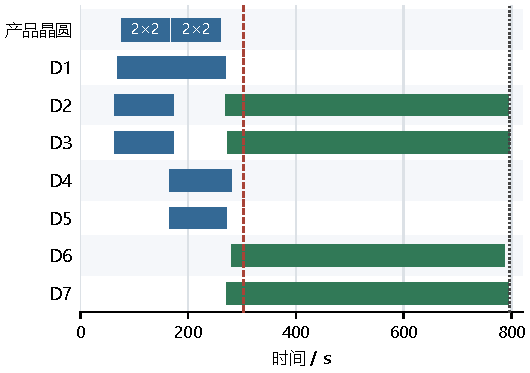
\includegraphics[width=\linewidth]{fig_coupled_schedule_merged_cn}
\caption{产品晶圆连续加工及辅助片借用区间。上行为产品晶圆的两次$2\times2$加工；D1--D7的蓝色、绿色区间分别表示生产、清洁用途的借用。虚线和点线分别表示303~s产品完工与796~s全部占用结束。}
\label{fig:d-coupled-witness-cn}
\end{figure}
\section{两阶段时序精修与节拍消融（配置E）}\label{sec:stage2-validation-cn}
配置E的30组阶段内配对均通过模型检查和物理重放；第一阶段270秒、精修30秒，同一次运行的前后解比较，全部保持产品完工上界。普通资格24次总等待降幅29.66\%至95.85\%，受限资格6次46.74\%至67.40\%；该指标累加产品和辅助晶圆的受计量路线等待，反映固定产品完工时间下的时序压缩。
\begin{table}[!htbp]
\centering\small
\caption{配置E同一排程的时序精修（三种子均值，单位：s）}
\label{tab:refinement-ablation-cn}
\resizebox{\columnwidth}{!}{%
\begin{tabular}{ccccc}\toprule
$N/H$ & 供片来源与腔室限制 & $C_{\max}$ & 精修前等待 & 精修后等待\\\midrule
4/3 & 单源 & 1491.00 & 1648.00 & 840.00\\
4/3 & 双源 & 854.53 & 3991.73 & 333.67\\
4/10 & 单源 & 1491.00 & 1185.00 & 600.00\\
4/10 & 双源 & 851.97 & 1259.65 & 626.67\\
8/3 & 单源 & 3933.00 & 3158.00 & 1680.00\\
8/3 & 双源 & 2071.00 & 10943.00 & 536.00\\
8/10 & 单源 & 2985.00 & 2276.00 & 1200.00\\
8/10 & 双源 & 1720.00 & 10998.02 & 692.00\\
8/3 & 单源、限制腔室 & 4707.00 & 3830.00 & 2040.00\\
8/3 & 双源、限制腔室 & 2264.00 & 1046.00 & 341.00\\
\bottomrule\end{tabular}}
\end{table}
\begin{table}[!htbp]
\centering\small
\caption{节拍权重消融（配置E，三种子均值，时间单位：s）}
\label{tab:rhythm-weight-cn}
\begin{adjustbox}{max width=\linewidth}
\begin{tabular}{lrrrr}\toprule
实例 & $\lambda$ & $C_{\max}$ & 总等待 & 节拍偏差\\\midrule
16片纯$2\times2$ & 0 & 2537 & 1000 & 792\\
 & 5 & 2537 & 1016 & 784\\
 & 25 & 2537 & 1016 & 784\\
 & 100 & 2537 & 1016 & 784\\
24片混合 & 0 & 5199 & 1440 & 20\\
 & 5 & 5199 & 1440 & 20\\
 & 25 & 5199 & 1440 & 20\\
 & 100 & 5199 & 1440 & 20\\
\bottomrule\end{tabular}
\end{adjustbox}
\par\smallskip\footnotesize 两实例分别含6个和2个有效节拍中心；各臂最大等待均为65~s。
\end{table}
上表的16/24片两个实例分别有6/2个节拍中心，三种子共享各自第一阶段结构，只改变权重；每臂60秒，24次均达到受限精修最优。16片实例的偏差由792降至784秒，总等待由1000增至1016秒，权重5、25和100的指标相同；24片实例在四档权重下均无变化。这一结果体现了等待压缩与节拍均衡的折中。D下另外9次要求至少两个节拍中心的搜索均未取得可行输入，后续权重消融未执行。
\section{供片与库存变化下的初始化和选割收益}
\label{sec:journal-transfer-cn}

\begin{table}[!t]
\centering\small
\caption{不同配方与供片场景下的算法对照（产品完工均值，s）}
\label{tab:journal-transfer-cn}
\begin{adjustbox}{max width=\linewidth}
\begin{tabular}{cccccccc}\toprule
配方 & 场景 & SCIP & HEM & RL-DMCT-S & SCIP+SPBS & HEM+SPBS & RL-DMCT\\\midrule
$4\times1$ & S1 & 324.00 & 324.00 & 324.00 & 324.00 & 324.00 & 324.00\\
$4\times1$ & S2 & 324.00 & 324.00 & 324.00 & 324.00 & 324.00 & 324.00\\
$4\times1$ & S3 & 324.00 & 324.00 & 324.00 & 324.00 & 324.00 & 324.00\\
$2\times2$ & S2 & 342.00 & 342.67 & 342.00 & 344.00 & 344.00 & 343.33\\
混合 & S2 & 521.00 & 520.00 & 520.11 & 492.00 & 492.00 & 492.00\\
混合 & S3 & 327.00 & 327.00 & 326.67 & 327.00 & 327.00 & 326.11\\
\bottomrule\end{tabular}
\end{adjustbox}
\end{table}

为检验初始化和选割在不同输入条件下的效果，本节改变供片分布与辅助库存，分别比较初始排程的改善，以及各选割组件从相同初始排程出发获得的进一步改善。

\paragraph{供片、清洁阈值与库存变化下的共同起点}

为考察不同配方与供片场景下的算法表现，将$N\in\{2,4,8\}$、三种配方与三个场景交叉，形成27个测试实例。场景S1将产品集中于LP1、$H=2$、辅助库存为4片；S2按LP1--LP4轮转分配产品、$H=3$、辅助库存为6片；S3将前半产品置于LP1、后半置于LP2、$H=5$、辅助库存为8片。各场景通过改变供片分布、清洁频率和辅助库存覆盖不同输入组合。使用SCIP在无初始解的条件下搜索可行排程，求解种子为17、名义预算为1200~s，得到六个2片实例的可行排程，资格覆盖为6/27，其余21例在预算内未取得可行解。后续算法对照使用这六份排程作为共同起点；初始解搜索时间与后续300~s改善预算分别统计。

在这六个2片实例上，采用正常分离，沿用多训练种子对照并增加三种带SPBS的消融变体。算法和共享准备生成的赋值均通过完整模型约束检查和独立物理重放。每个实例与求解种子组合执行一次共享SPBS，共得到18份初始排程，其中3份降低产品完工时间；同组所有带SPBS的方法使用相同排程。209次运行证明完整主问题最优，205次取得限时可行解，实际主求解均未超过设定预算。

\paragraph{初始化收益随输入结构和预算分配变化}

如表~\ref{tab:journal-transfer-cn}所示，三个纯$4\times1$实例在各方法下均证明324~s最优。混合S2的原输入为521~s，共享SPBS分别给出494、494、488~s，均值492~s；各方法均保留这些起点，因此该实例的改善来自初始化。混合S3的共享起点均为327~s，RL-DMCT进一步将均值降至326.11~s，而HEM加SPBS保持327~s。纯$2\times2$ S2上，RL-DMCT的343.33~s低于HEM加SPBS的344~s，但高于无SPBS时的342~s；该实例初始化未改善起点，同时缩短了后续主求解时间。结合第~\ref{sec:journal-training-cn}节的结果，SPBS对部分混合实例形成了有效起点，其收益随输入结构及预算分配而变化。

\paragraph{共享初始解后选割组件带来的额外改善}

表~\ref{tab:journal-transfer-components-cn}给出了共享SPBS输入后的组件对照。对RL-DMCT与HEM加SPBS按同一实例、训练种子和求解种子配对，先在实例内平均相对完工时间差，再对各实例等权汇总，平均改善为0.0776\%，中位数为0，2胜、4平。按实例重采样的描述性95\%区间为$[0,0.1682]\%$。三个训练种子的实例平均改善依次为0.0510\%、0.1309\%和0.0510\%。

\begin{table}[!htbp]
\centering\small
\caption{共享SPBS输入的组件对照（产品完工均值，s）}
\label{tab:journal-transfer-components-cn}
\resizebox{\columnwidth}{!}{%
\begin{tabular}{ccccc}\toprule
方法 & 三个纯$4\times1$ & $2\times2$ S2 & 混合S2 & 混合S3\\\midrule
HEM+SPBS & 324.00 & 344.00 & 492.00 & 327.00\\
仅扩展特征+SPBS & 324.00 & 344.00 & 492.00 & 326.67\\
去结构重排+SPBS & 324.00 & 344.00 & 492.00 & 327.00\\
贪心替代束搜索+SPBS & 324.00 & 344.00 & 492.00 & 326.67\\
RL-DMCT & 324.00 & 343.33 & 492.00 & 326.11\\
\bottomrule\end{tabular}}
\end{table}

表~\ref{tab:journal-transfer-components-cn}中，完整组合在纯$2\times2$ S2和混合S3上的平均完工时间均低于三种消融变体，其余四实例持平。相较仅扩展特征、去结构重排和贪心替代束搜索，六实例平均配对改善分别为0.0605\%、0.0776\%和0.0606\%。结合第~\ref{sec:journal-ablation-cn}节根分离下贪心替代束搜索结果更好的对照可见，完整选割组合在共享起点后取得了额外改善，束搜索的收益则依赖求解设置。


\section{满片加工与共享资源约束的排程验证}
\label{sec:coverage-scale-cn}

本节通过两份完整排程展示设备执行过程：2片实例的最优排程说明辅助片如何补足满片加工所需工位，16片实例的可行排程展示两腔如何共用搬运资源。两份排程均通过完整模型约束检查和独立事件时序验证。

\subsection{2片最优排程中的辅助片补位}

图~\ref{fig:small-optimal-gantt-cn}给出2片同LP纯$4\times1$实例的一份产品完工时间最优排程。两片产品均属于Pjob1且由LP1供片，辅助库存为8片，清洁阈值为3。主问题下界与排程的产品完工时间均为324~s，因此该排程在产品完工时间目标下达到全局最优。

\begin{figure}[!htbp]
\centering
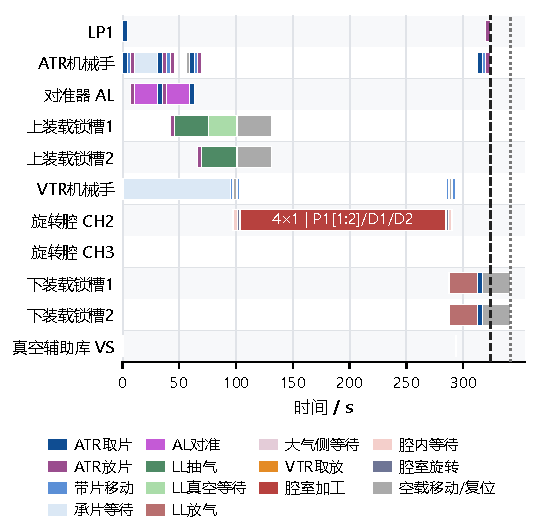
\includegraphics[width=\columnwidth]{fig_schedule_n2_cn}
\caption{2片同LP纯$4\times1$产品的完工时间最优排程。P1[1:2]表示Pjob1的两片产品，D1、D2为辅助片。虚线与点线分别标示324~s产品回片和342~s全部占用结束。}
\label{fig:small-optimal-gantt-cn}
\end{figure}

该排程以两片产品组成一个PW对，以辅助片D1、D2组成另一个PW对，共同填满CH2的四个工位，并在104--284~s完成180~s加工。产品片依次经过ATR搬运、对准器和上装载锁，由VTR装入腔室；辅助PW对先于产品PW对装入，使加工开始时满足满片条件。加工结束后，产品经下装载锁返回LP1，辅助片于294~s归还真空辅助库。

两片产品均于324~s回到LP1，下装载锁的压力复位持续至342~s。该排程展示了产品数量不足四片时的辅助片补位与完整取还流程，并区分了产品回片和设备复位两个结束时刻。腔室仅执行一个加工周期，未达到清洁阈值。

\subsection{16片可行排程中的双腔加工与搬运安排}

图~\ref{fig:current-defaults-gantt-cn}展示16片纯$4\times1$产品的可行排程。四个LP各含4片产品，均属于Pjob1并可进入CH2与CH3；辅助库存为8片，清洁阈值为3。

\begin{figure}[!htbp]
\centering
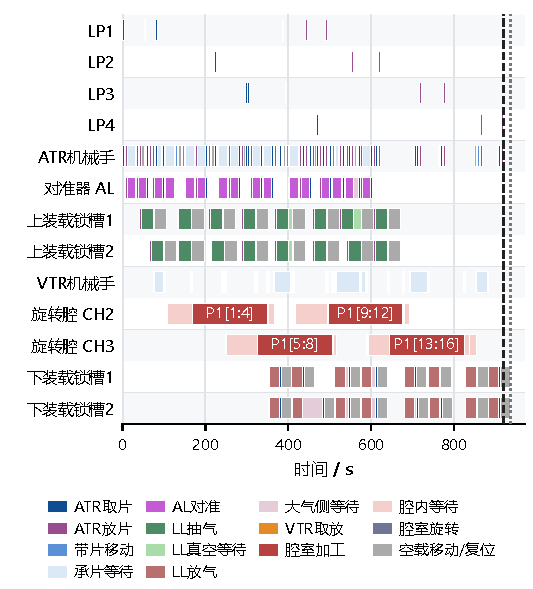
\includegraphics[width=\columnwidth]{fig_schedule_n16_cn}
\caption{16片纯$4\times1$产品的完整资源可行排程。LP1--LP4各含4片产品，均属于Pjob1。虚线与点线分别标示920~s产品回片和938~s全部占用结束。}
\label{fig:current-defaults-gantt-cn}
\end{figure}

该排程以预先构造的晶圆动作序列为输入，将其配对、腔室分配及事件时刻代入完整模型进行可行性检验。模型包含64个候选PW对、每腔32个候选周期，共177905个变量与671864条约束。全部赋值满足产品可加工腔室限制、有限资源容量、非加工驻留及同任务非递减投片约束，独立事件时序验证也通过。

该排程的产品完工时间为$C_{\max}=920$~s，16片产品组成8个PW对，共执行4个满片周期。CH2于170--350~s与497--677~s分别加工Pjob1的第1--4片和第9--12片；CH3于326--506~s与645--825~s分别加工第5--8片和第13--16片。每片均完成一次180~s工艺处理，按已验证的搬运与装载锁流程返回原LP。

图~\ref{fig:current-defaults-gantt-cn}给出152个事件的时间安排，包括LP取还、ATR、对准器、上下装载锁、VTR以及两工艺腔的占用。腔室加工可与其他产品的供片和回片搬运同时进行，各PW对的搬运次序受共享机械手与装载锁约束。全部产品于920~s回到LP，下装载锁的压力复位持续至938~s，产品完工与全部占用结束相差18~s。每腔仅加工两个周期，尚未达到清洁阈值3；全部周期由产品片满载，未借用辅助片。该排程展示了满片条件下两腔加工与共享资源的使用次序。


\FloatBarrier
\section{100片完整排程与模型适用边界}
历史固定结构模型保存了100片混合配方的有效排程，其中50片为$4\times1$、50片为$2\times2$，产品完工时间为9998秒。该结果保存了原模型独立赋值检查，属于可行解，未证明全局最优。其工艺计时、辅助片配置与候选结构不同于本章默认配置D，因此仅作为既有大规模排程的历史示例，不纳入D的性能排名。默认配置D的75片混合批次见第~\ref{sec:pareto-evidence}~节，100片完整对照仍待验证。

图~\ref{fig:legacy100a}和图~\ref{fig:legacy100b}按产品编号分两页展示全部100片的轨迹，附图保留原始SVG中各动作的起止时刻；完整辅助片与资源视角随论文资料包保存。
\begin{figure}[p]\centering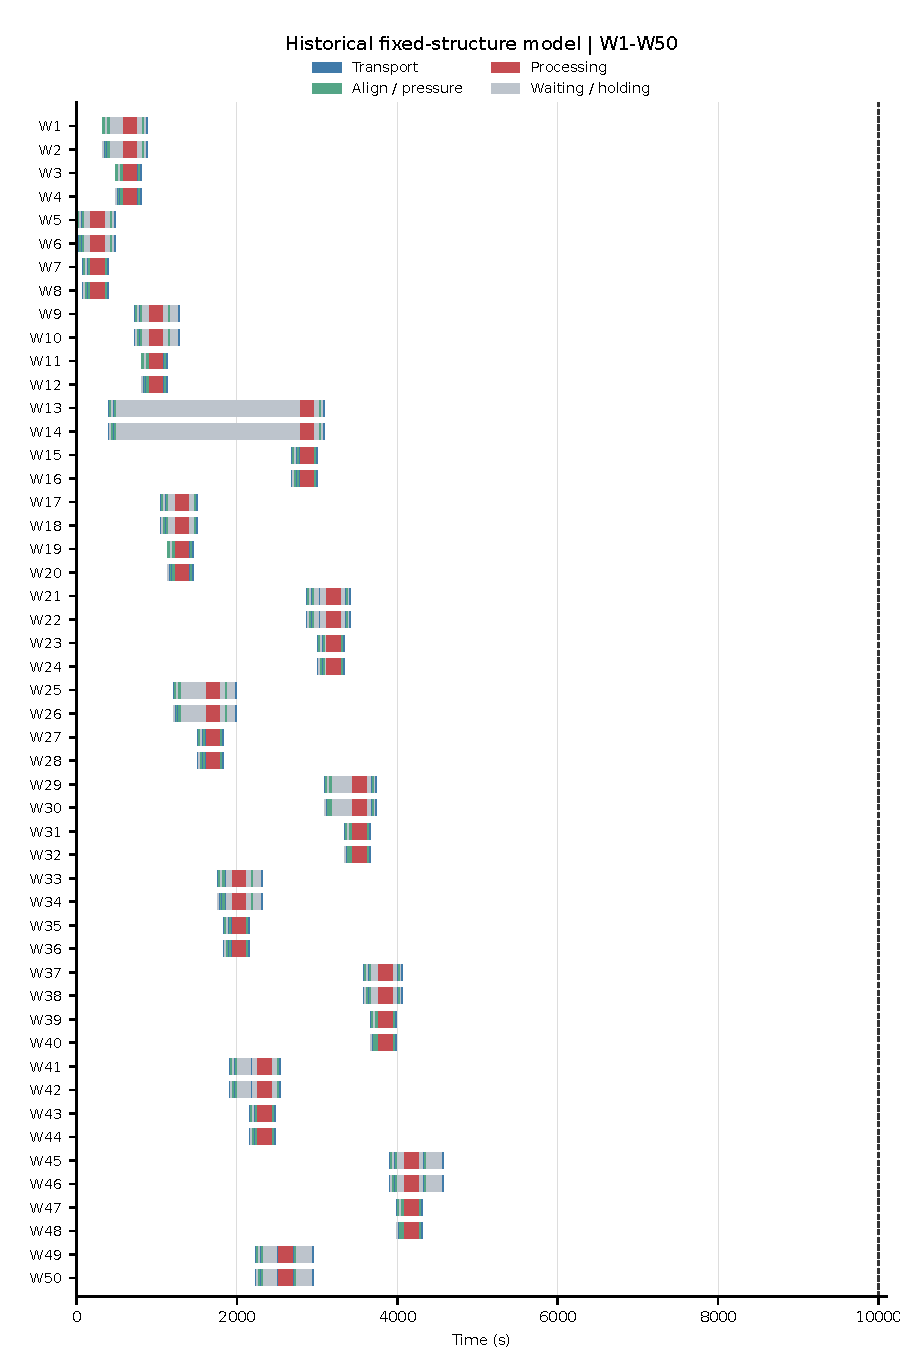
\includegraphics[width=\linewidth,height=0.84\textheight,keepaspectratio]{legacy100_products_1}\caption{历史固定结构模型100片混合排程：产品1至50（全部时间轴）}\label{fig:legacy100a}\end{figure}
\begin{figure}[p]\centering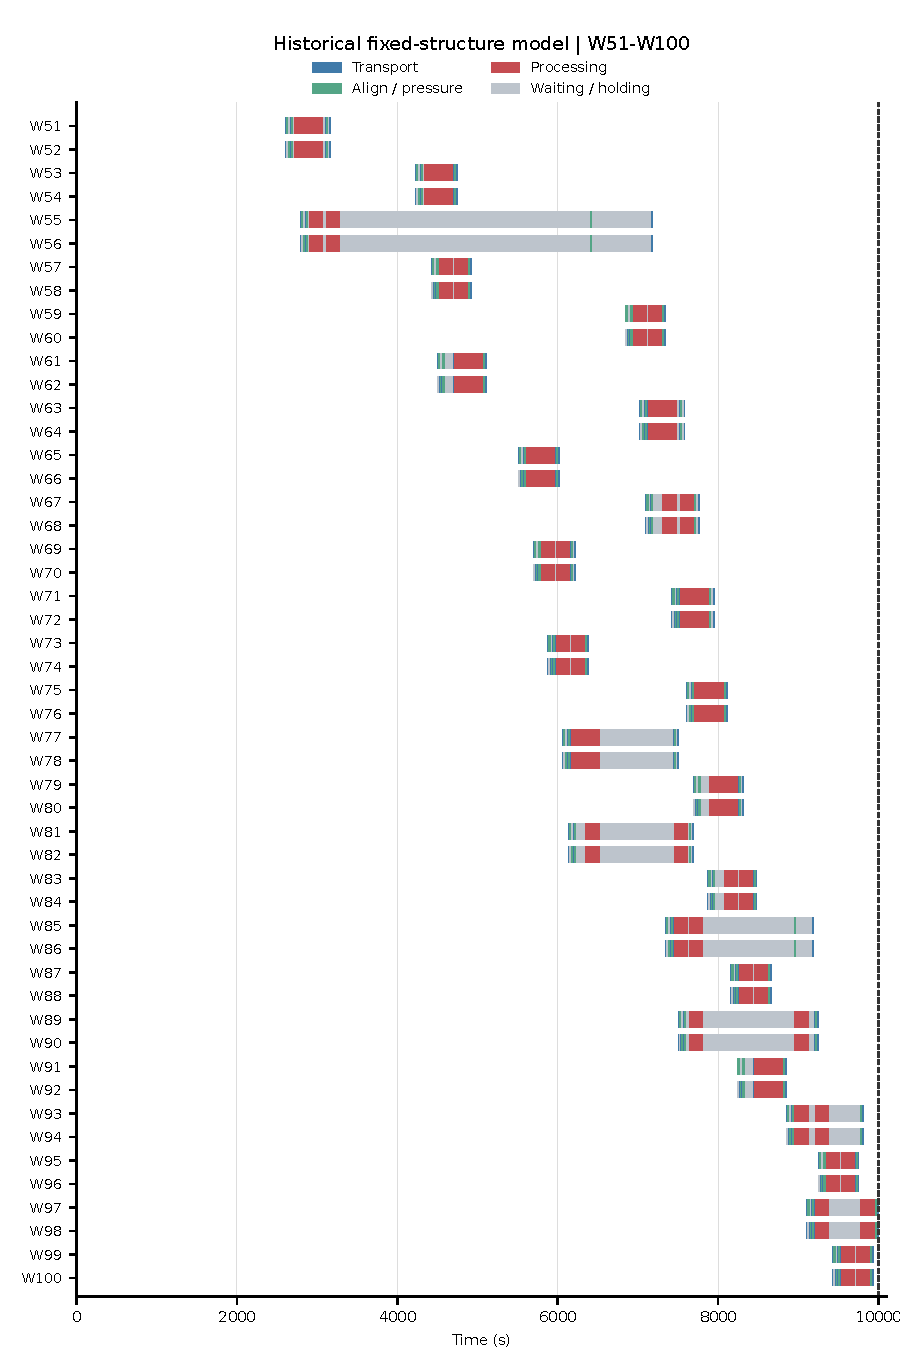
\includegraphics[width=\linewidth,height=0.84\textheight,keepaspectratio]{legacy100_products_2}\caption{历史固定结构模型100片混合排程：产品51至100（全部时间轴）}\label{fig:legacy100b}\end{figure}
\FloatBarrier

\clearpage
\section{双目标前沿、组件消融与75片排程}\label{sec:pareto-evidence}

\subsection{两目标的冲突与可认证前沿}

两片算例S1含同一Pjob的两片$2\times2$产品、四片辅助片，清洁阈值为2。采用该工况的配对与双腔时序子模型，在82.03~s内重新生成图~\ref{fig:pareto-s1}的七份排程。逐点重放并与独立数值证书比对，在$2\times10^{-5}$容差内命中七个全局非支配点，含三个非支持点。最快回片为331~s，对应$B=424/3$。最低$B=42$对应519~s。当上限为$B\le100$时，两片分别与辅助片配对，最短工期为514~s。只从线性加权和的支持点中选解则需519~s。该例的$R=0$，两目标的冲突来自交付与路线等待。专用重算的HV为0.378339，$\mathrm{IGD}^{+}=2.45\times10^{-10}$。通用领域搜索在40~s内每个种子命中一个认证点，种子1延长至300~s后命中两个点。
\begin{figure}[!htbp]
\centering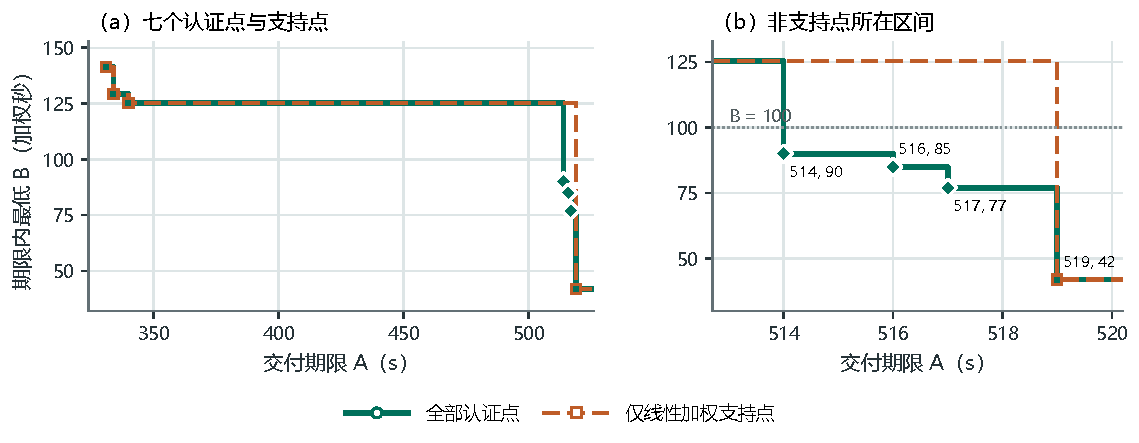
\includegraphics[width=.92\linewidth]{pareto_s1}
\caption{两片算例S1的七个认证点及线性加权和的四个支持点。阶梯给出交期内可达的最低指标，右图放大含三个非支持点（菱形）的区间。}\label{fig:pareto-s1}
\end{figure}

四片标称混合工况M4中，发现了413~s交付的排程。已证最低$B$为54，达到该值至少需要476~s，已验证排程将对应的最短工期限定在$[476,497]$~s。因此追求最低$B$至少要比413~s的排程多等63~s。在已访问的35种整数结构中，开放连续时刻后有一段位于这些结构合并边界上的有效线段，其工期区间为$(420.5,423)$~s。该区间的结论限于这35种结构。

\subsection{等预算对照与扰动}

五个工况各比较六种方法，每个方法使用三个种子。S1、M4、H4、H8和H16的产品组成（$4\times1$片数，$2\times2$片数）依次为$(0,2)$、$(2,2)$、$(3,1)$、$(4,4)$和$(8,8)$。同工况、同种子的各臂共享可行起点。NSGA-II采用非支配排序与拥挤距离选择\citep{deb2002}，MOEA/D采用切比雪夫分解与邻近权重子问题替换\citep{zhangli2007}。两种基线以Python实现并共用设备解码器。$\varepsilon$-SCIP直接在原模型中扫描目标上限，原两阶段法保持工期优先。表~\ref{tab:pareto-small}给出各方法返回集合的超体积（HV）中位数。对归一化的双目标计算该集合支配至参考点$(1.1,1.1)$的面积，数值越大表示覆盖越广。S1按认证前沿极值定标，其他工况按共同起点$(A_0,B_0)$取$[0,1.5A_0]\times[0,2B_0]$。HV在同一工况内比较。
\begin{table}[!htbp]\centering\small
\caption{五个工况的三种子HV中位数与单次搜索时限}\label{tab:pareto-small}
\begin{tabular}{lrrrrrrr}\toprule
工况 & 时限/s & 领域搜索 & 加选割 & $\varepsilon$-SCIP & NSGA-II & MOEA/D & 两阶段 \\\midrule
S1 & 40 & 0.27468 & 0.27468 & 0.00000 & 0.27468 & 0.27468 & 0.00000 \\
M4 & 45 & 0.54479 & 0.54116 & 0.26126 & 0.53952 & 0.53947 & 0.35375 \\
H4 & 45 & 0.75582 & 0.75448 & 0.26000 & 0.70736 & 0.70690 & 0.35386 \\
H8 & 55 & 0.58856 & 0.58856 & 0.26000 & 0.57961 & 0.61188 & 0.28050 \\
H16 & 80 & 0.37344 & 0.38830 & 0.26000 & 0.47203 & 0.50191 & 0.26000 \\
\bottomrule\end{tabular}
\end{table}

领域搜索在两种四片混合工况的HV中位数均最高。八片、十六片工况由MOEA/D取得最高中位数。用同一随机种子配对比较，M4开启配对下界、在已有下界时采用领域邻域、允许改变对内取放顺序，对应的HV差值中位数分别为$+0.00372$、$+0.01710$和$+0.06650$，三项改动在三个种子中均提高HV。自适应选择上限的差值为$-0.02102$，接入冻结选割策略的差值为$-0.00330$。在12对固定上限、共享起点的4~s原模型子问题中，下界对其中6对排除了至少一种配对数量，12对的条件工期均相同。

M4另将邻域释放比例从0.30分别改为0.15和0.50，两个配对种子的HV差值中位数分别为$-0.03107$和$-0.02767$。把修复预算比例从0.22改为0.12和0.32，对应变化为$-0.00734$和$+0.00105$。在八片节拍实验R8中，151份归档排程有46份产生非零节拍偏差。对同批候选在相同工期上限下分别按0、12.5、25和50重算节拍权重，五个有可选排程的种子与工期上限组合均选择了相同的$R$值。这些数据区分了节拍项实际激活与改变权重后决策发生变化两种情况。

\subsection{75片混合批次的可行前沿}

采用默认配置D，37片执行$4\times1$，38片执行$2\times2$。LP1至LP4的两类产品数量分别为$(10,9)$、$(9,10)$、$(9,10)$和$(9,9)$。两个Pjob共用CH2和CH3，真空辅助库存为8片，清洁阈值为3，时域为10000~s。历史构造得到的可行起点为$(A_0,B_0)=(8630,3932)$。四种方法由同一起点出发，各运行三个种子，每次限时90~s。共享起点的外部准备与完整原模型的事后复核单独计时，搜索时限包含结构调整、重定时和设备事件复验。固定结构对照仅改变动作时刻及$B$上限，在预设网格的扫描区间耗尽后提前停止。

每次运行按预设规则提交至多七点，先保留两个端点，再依次选择与已保留集合的归一化距离最大的点。表~\ref{tab:pareto75}的HV仅使用当次提交点。最后两列分别对各次提交集合的最小$A$与最小$B$取中位数，两列可以对应不同的排程。
\begin{table}[!htbp]\centering\small
\caption{75片混合批次的三种子结果。HV范围为三次运行的最小值至最大值。}\label{tab:pareto75}
\begin{tabular}{lrrrr}\toprule
方法 & HV中位数 & HV范围 & 最小$A$/s & 最小$B$/加权秒 \\\midrule
领域搜索 & 0.44494 & 0.44391--0.44546 & 7623 & 1786 \\
NSGA-II & 0.43287 & 0.41437--0.43561 & 7586.88 & 1951 \\
MOEA/D & 0.43898 & 0.43789--0.44693 & 7662 & 1851.5 \\
固定结构扫描 & 0.27137 & 0.27137--0.27137 & 8630 & 3722 \\
\bottomrule\end{tabular}
\end{table}

领域搜索的HV中位数为0.44494，MOEA/D为0.43898。第二个种子中MOEA/D取得0.44693，高于同种子的领域搜索。固定生产块和资源次序后，单靠重定时仍能在$(8630,3932)$与$(8852,3722)$之间找到取舍。开放结构后的三个搜索方法均改善了固定结构法的中位HV。75片领域搜索在本组所用上限上未触发配对下界筛除，表中差异不能归因于该下界或学习选割。

图~\ref{fig:pareto75}的黑色点线汇集原90~s实验各方法发现的非支配解，含单次提交时被七点上限省略的内部点。按两目标再次去支配后共得20个实际坐标。在最短工期端，$(A,B)=(7567,2599)$。在最低等待与节拍指标端，$(A,B)=(8045,1782)$。从前者换到后者，批次晚交付478~s，$B$减少817加权秒。若只在本次候选中选择，要求$B\le2000$时最早可在7639~s交付。该值可与两端点一起用于选择交期。
\begin{table}[!htbp]\centering\small
\caption{75片共同起点与按交付要求选取的三份排程。$A$、$L_{\rm sum}$、$L_{\max}$和$R$的单位为秒，$B$为加权秒。}\label{tab:pareto75-policies}
\begin{tabular}{lrrrrr}\toprule
排程选择 & $A$ & $B$ & $L_{\rm sum}$ & $L_{\max}$ & $R$ \\\midrule
共同起点 & 8630 & 3932 & 3312 & 62 & 0 \\
发现的最短工期 & 7567 & 2599 & 1884 & 49 & 9 \\
$B\le2000$时最早交付 & 7639 & 1951 & 1776 & 17.5 & 0 \\
发现的最低$B$ & 8045 & 1782 & 1612 & 17 & 0 \\\bottomrule
\end{tabular}
\end{table}
\FloatBarrier
\begin{figure}[!htbp]
\centering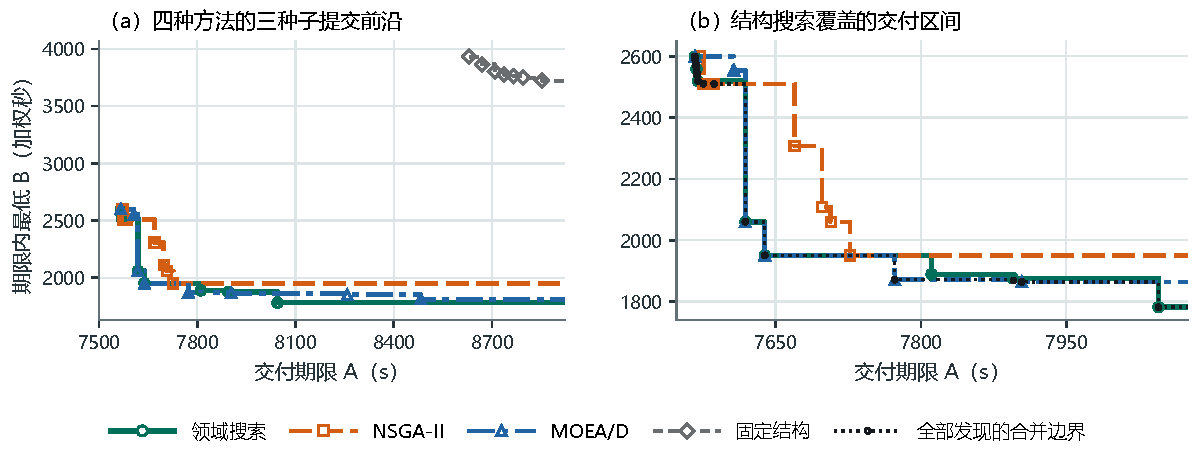
\includegraphics[width=.96\linewidth]{pareto_75}
\caption{37+38片限时实验的经验前沿。左图按方法合并三个种子的提交点，右图放大较早交付的区间，黑色点线纳入所有方法未截断的内部档案。}\label{fig:pareto75}
\end{figure}

两端点的排程均含九个可计量的节拍位置。沿最短工期端到最低$B$端，总等待由1884降至1612~s，最大单项等待由49降至17~s，节拍偏差由9降至0~s。三项分别解释$B$下降量中的272、320和225加权秒。

该90~s实验提交了78份排程。对提交集合及补全后的合并前沿去重，共有63份排程逐片重放，并向原模型的6\,764\,011个变量赋值、逐一检查24\,271\,470条约束。按事件复算的$A$、$B$与原模型赋值相符。小规模主比较、消融、参数扰动和长预算实验提交的699份最终排程均已核对。小规模的完整性证书仅适用于S1。75片的网格、有限结构邻域与搜索预算限定了本图的覆盖范围。对完整可行域尚无排除其他非支配点的证书。

\subsection{共享初始结构后的同预算比较}\label{sec:pareto75-paired}

三种子限时实验中，领域搜索先评价六类预设取放结构，两个进化算法从随机种群开始。为考察相同起点下的搜索效果，保留上述37片并行配方与38片链式配方的工况，并增加50片并行配方与25片链式配方的工况。后者从LP1至LP4分别供给$(13,6)$、$(13,6)$、$(12,7)$、$(12,6)$片产品，共同可行起点为$(8553,4274)$。其余设备、时间和库存参数保持一致。

比较领域搜索、均匀选片消融、NSGA-II及MOEA/D。均匀选片只改变选择待调整产品的概率。每种方法先对同一组六类结构各评价两个目标端点，再按各自规则搜索，合计160次候选评价，仍按同一规则提交至多七点评价HV。两种工况均使用种子101--112，并以固定结构扫描作为参照。图~\ref{fig:pareto75-paired-lines}上排给出预先固定的首个种子。对任一交期，先在每次运行的提交点中取能按时交付的最低$B$，再求至少半数种子能够达到的最低值，得到下排的50\%经验达到边界\citep{fonseca2011eaf}。达到该交期的种子不足半数时，曲线留空。

\begin{figure}[!htbp]\centering
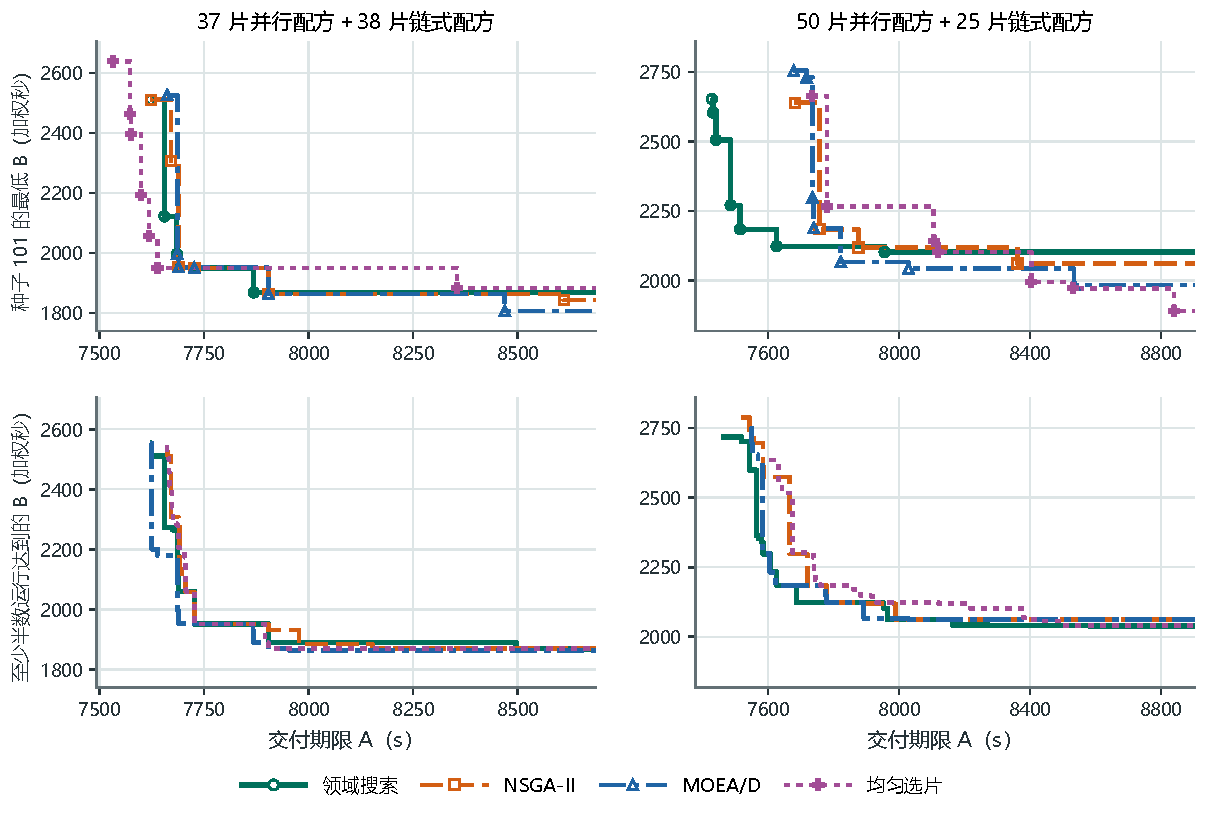
\includegraphics[width=.96\linewidth]{paired75_lines}
\caption{相同初始结构和评价预算下的75片前沿。上排符号为种子101实际提交的排程，阶梯表示该方法在给定交期内达到的最低$B$。下排为各方法的50\%经验达到边界。}\label{fig:pareto75-paired-lines}
\end{figure}

\begin{table}[!htbp]\centering\small
\caption{共享初始化下的单次提交HV中位数。产品组成按并行配方、链式配方计数。}\label{tab:pareto75-paired}
\begin{tabular}{lrrrr}\toprule
产品组成 & 领域搜索 & 均匀选片 & NSGA-II & MOEA/D \\\midrule
37+38 & 0.43990 & 0.43814 & 0.43989 & 0.44145 \\
50+25 & 0.44239 & 0.43686 & 0.43643 & 0.43902 \\
\bottomrule\end{tabular}
\end{table}

表~\ref{tab:pareto75-paired}中，37+38片的最高HV中位数来自MOEA/D，50+25片则来自领域搜索。在37+38片工况，按同一种子的提交HV比较，领域搜索对NSGA-II为7胜、0平，对MOEA/D为5胜、0平。在50+25片工况，对NSGA-II为8胜、0平，对MOEA/D为8胜、0平。对MOEA/D的两组比较中，分别有9组和10组双方都能给出对方无法同时改善的排程。以单次提交HV为主指标，对两个工况中领域搜索与三种对照的六个配对差异进行双侧精确符号检验，经Holm校正后最小$p$为0.876\citep{holm1979}。因此这两种工况下未观察到对通用算法的一致优势。相对均匀选片，优先调整长驻留产品在37+38片工况为8胜、0平，在50+25片工况为9胜、0平。其增量也未达到上述检验的显著水平。

\subsection{局部生产块调整的作用与可选排程}\label{sec:pareto75-mechanisms}

机制消融采用种子301--312，在每个工况比较三种搜索设置。第一组保留完整领域搜索。第二组仍可切换六类整体取放结构和优化动作时刻，关闭对个别生产块的局部改动。第三组保留局部改动，将六类预设初始结构替换为六个随机结构，仍各评价两个端点。三组使用相同的起始可行排程、160次候选评价及归档规则。在这一独立批次内对四项配对比较作Holm校正。

\begin{table}[!htbp]\centering\small
\caption{75片机制消融。差值为同一种子完整方法的HV减去消融方法的HV，正值表示保留该机制有利。}\label{tab:pareto75-mechanism}
\begin{tabular}{llrrrr}\toprule
产品组成 & 消融方式 & 胜 & 平 & HV差值中位数 & 校正后$p$ \\\midrule
37+38 & 关闭局部块调整 & 12 & 0 & $+0.01132$ & 0.00195 \\
37+38 & 改用随机初始结构 & 7 & 0 & $+0.00130$ & 1.00000 \\
50+25 & 关闭局部块调整 & 12 & 0 & $+0.02651$ & 0.00195 \\
50+25 & 改用随机初始结构 & 5 & 0 & $-0.00270$ & 1.00000 \\
\bottomrule\end{tabular}
\end{table}

表~\ref{tab:pareto75-mechanism}显示，保留局部生产块调整在两种工况中均为12胜、0平。用未截断的内部档案重算HV，结果相同。允许改变少数块的分腔、配对或取放次序，使后续重定时能访问仅切换整体结构时遗漏的交付与等待组合。该消融测量四类局部动作的合计收益。从同批运行的中间记录截取前80次评价，保留局部调整在两个工况仍均为12胜、0平。将160次评价的归一化HV参考点从$(1.1,1.1)$分别改为$(1.0,1.0)$和$(1.2,1.2)$，两种设置下的胜、平计数均相同。更换六类初始结构所得差值在两个工况中方向不一。

\begin{figure}[!htbp]\centering
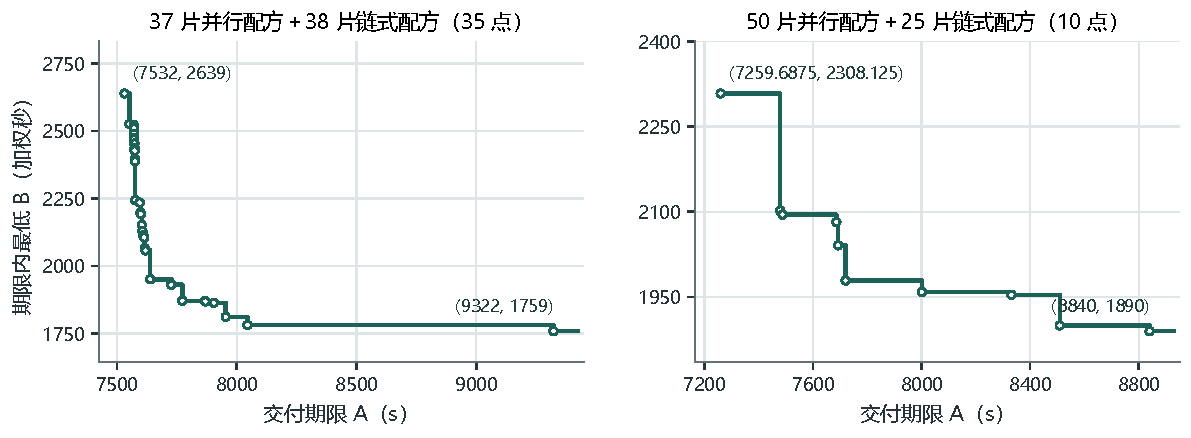
\includegraphics[width=.96\linewidth]{engineering75}
\caption{两种75片工况已发现的可行交付方案。合并同一工况全部实验的内部档案后去支配，圆点对应逐片复验的排程，阶梯给出交期内已达到的最低$B$。}\label{fig:pareto75-engineering}
\end{figure}

两轮补充实验共核验698份不同的完整排程。两种工况分别向原模型的$6\,764\,011$和$5\,661\,546$个变量赋值，逐份检查$24\,271\,470$和$20\,611\,580$条约束。图~\ref{fig:pareto75-engineering}合并同一工况的各方法、种子和实验批次，37+38片还纳入原90~s实验，分别得到35和10个经验非支配点。若要求$B\le2000$，两种工况在已发现排程中最早可于7639和7720~s交付，对应的$B$分别为1951和1979。每个点均可回溯至完整排程，两种工况的全局前沿仍待认证。
\FloatBarrier

\chapter{总结与未来展望}
\section{研究总结}
本文以PW对连接成对搬运与腔室周期。两阶段MILP先最小化产品完工时间，再固定完工上界和主要结构改进时序。配置E的30组对照均保持工期并降低等待。配置D的单产品链式工况将总等待由642降至54~s。权重变化使16片实例以16~s额外等待换取8~s节拍偏差下降，24片实例保持不变。

正常分离实验中，两个混合实例在三个训练种子下均从结构化初始化获益。场景S2的平均工期由521降至492~s。共享SPBS起点后，完整选割组合相对HEM加SPBS的实例平均配对改善为0.0776\%，2胜、4平。根分离下贪心解码优于束搜索，表明收益随解码设置变化。

单产品链式工况的辅助库存从4片增至8片，已证最优工期由309降至303~s，并行配方保持296~s。四片辅助片可通过重复借用完成链式加工与满片清洁。身份、原模型与事件复核验证了2片324~s最优排程和16片920~s可行排程。

\section{交付与路线等待的双目标权衡}
配对等待下界把指标上限转化为结构筛选条件。两片算例的七个认证点含三个非支持点。四片标称实例的配对下界、领域邻域和对内取放改动均提高了三个种子的超体积。八片与十六片由MOEA/D取得最高HV中位数。两种75片配方组合分别得到35和10个经验非支配点。相同初始结构与160次候选评价下，领域搜索相对两个进化基线的差异未达显著水平。相较关闭局部生产块调整，完整方法在两种工况均为12胜、0平，HV配对差值中位数分别为0.01132和0.02651。大批次实验支持将局部块调整与重定时结合以扩大交付和等待的可选范围。

\section{未来展望}
75片经验前沿仍受生产块和离散次序邻域限制。后续可用工期与等待的联合下界逐段排除未知区间，并在更多配方比例、辅助库存和清洁阈值下检验大批次的前沿覆盖度。向配置D的100片批次扩展时，还需测量构造、构模、搜索与验解的总耗时。

\begingroup
\renewcommand{\bibfont}{\zihao{5}}
\setlength{\bibsep}{0pt}
\setstretch{1.3}
\cleardoublepage\phantomsection\addcontentsline{toc}{chapter}{参考文献}
\begin{thebibliography}{48}
% 按全篇首次引用顺序排列。
\interlinepenalty=10000

\bibitem{appliedprecisioncvd}
Applied Materials. Producer XP Precision CVD.
n.d.
\url{https://www.appliedmaterials.com/us/en/product-library/producer-xp-precision-cvd.html} (accessed September 7, 2026).

\bibitem{pan2018survey}
Pan CR, Zhou MC, Qiao Y, Wu NQ. Scheduling cluster tools in semiconductor manufacturing: Recent advances and challenges.
IEEE Trans Autom Sci Eng 2018;15:586--601.
\url{https://doi.org/10.1109/TASE.2016.2642997}.

\bibitem{gu2024multifinger}
Gu L, Wu N, Qiao Y, Zhang S. Scheduling of {Multi-finger-robotic Cluster Tools} with {Multi-space Process Modules}.
In: 2024 International Conference on Networking, Sensing and Control ({ICNSC}). IEEE; 2024.
\url{https://doi.org/10.1109/ICNSC62968.2024.10760109}.

\bibitem{perkinson1994throughput}
Perkinson TL, McLarty PK, Gyurcsik RS, Cavin RK. Single-wafer cluster tool performance: An analysis of throughput.
IEEE Trans Semicond Manuf 1994;7:369--73.
\url{https://doi.org/10.1109/66.311340}.

\bibitem{rostami2002optimal}
Rostami S, Hamidzadeh B. Optimal scheduling techniques for cluster tools with process-module and transport-module residency constraints.
IEEE Trans Semicond Manuf 2002;15:341--9.
\url{https://doi.org/10.1109/TSM.2002.801379}.

\bibitem{wu2010closedform}
Wu NQ, Zhou MC. A closed-form solution for schedulability and optimal scheduling of dual-arm cluster tools with wafer residency time constraint based on steady schedule analysis.
IEEE Trans Autom Sci Eng 2010;7:303--15.
\url{https://doi.org/10.1109/TASE.2008.2008633}.

\bibitem{qiao2014revisiting}
Qiao Y, Wu N, Zhou MC. Scheduling of dual-arm cluster tools with wafer revisiting and residency time constraints.
IEEE Trans Ind Inform 2014;10:286--300.
\url{https://doi.org/10.1109/TII.2013.2272702}.

\bibitem{qiao2015thesis}
乔岩. 半导体制造中组合设备的建模、优化调度与控制 [D]. 广州：广东工业大学，2015.

\bibitem{zhou2022thesis}
周家忠. 基于时间Petri网离散事件系统的优化调度 [D]. 西安：西安电子科技大学，2022.

\bibitem{yuan2023survey}
袁凤连，黄波，王际鹏，潘春荣. 基于Petri网的组合设备建模与调度综述. 自动化学报，2023，49(5)：929--948.
\url{https://doi.org/10.16383/j.aas.c210951}.

\bibitem{wang2020multiple}
Wang J, Hu H, Pan C, Zhou Y, Li L. Scheduling dual-arm cluster tools with multiple wafer types and residency time constraints.
IEEE/CAA J Autom Sin 2020;7:776--89.
\url{https://doi.org/10.1109/JAS.2020.1003150}.

\bibitem{ko2021balance}
Ko SG, Yu TS, Lee TE. Wafer delay analysis and workload balancing of parallel chambers for dual-armed cluster tools with multiple wafer types.
IEEE Trans Autom Sci Eng 2021;18(3):1516--1526.
\url{https://doi.org/10.1109/TASE.2021.3061140}.

\bibitem{yang2025miptwowafers}
Yang F, Li C, Zhen L, Zhang C, Wu N. Scheduling residency time-constrained single-armed cluster tools with two-wafer types via mixed integer programming model.
Expert Syst Appl 2025;288:128209.
\url{https://doi.org/10.1016/j.eswa.2025.128209}.

\bibitem{li2023urgent}
李金成，潘春荣. 面向单臂组合设备中紧急订单的调度. 信息与控制，2023，52(5)：626--637.
\url{https://doi.org/10.13976/j.cnki.xk.2023.2303}.

\bibitem{luo2026mask}
罗亚波，巫琳，张峰. 考虑换模操作的双臂组合设备终止暂态调度. 工业工程，2026，29(1)：120--132.
\url{https://doi.org/10.3969/j.issn.1007-7375.240320}.

\bibitem{yang2025noncyclic}
Yang F, Xu X, Yang Z, Li C, Zhen L, Wu N. Non-cyclic scheduling of single-armed cluster tools for processing two wafer types.
IEEE Trans Autom Sci Eng 2025;22:14133--14146.
\url{https://doi.org/10.1109/TASE.2025.3554273}.

\bibitem{kim2023tandemphd}
Kim T. Scheduling and control of tandem cluster tools [D]. Daejeon: Korea Advanced Institute of Science and Technology, 2023.
\href{https://library.kaist.ac.kr/search/detail/view.do?bibCtrlNo=1046815&flag=dissertation}{KAIST Library, DIE~23014}.

\bibitem{pan2024twin}
潘春荣，周浩，熊文清，崔煜，罗继亮. 晶圆驻留时间约束下双组合设备协同调度. 信息与控制，2024，53(6)：804--816.
\url{https://doi.org/10.13976/j.cnki.xk.2024.3457}.

\bibitem{jee2021thesis}
Jee YJ. Scheduling of multi-slot cluster tools with wafer delay constraints [D]. Daejeon: Korea Advanced Institute of Science and Technology, 2021.
\href{https://library.kaist.ac.kr/search/detail/view.do?bibCtrlNo=956468&flag=dissertation}{KAIST Library, DIE~21004}.

\bibitem{zou2024twospace}
Zou C, Wang G, Gu L, Li J, Wu N, Qiao Y. Scheduling of time-constrained single-arm cluster tools with two-space process modules in semiconductor manufacturing.
IEEE Robot Autom Lett 2024;9(7):6352--6359.
\url{https://doi.org/10.1109/LRA.2024.3396112}.

\bibitem{huang2025efem}
Huang B, Wu N, Qiao Y, Guo W. Scheduling single-arm cluster tools with an equipment front-end module subject to wafer residency time constraints.
IEEE Trans Autom Sci Eng 2025;22:9544--9558.
\url{https://doi.org/10.1109/TASE.2024.3507854}.

\bibitem{yu2020delay}
Yu TS, Lee TE. Wafer delay analysis and control of dual-armed cluster tools with chamber cleaning operations.
Int J Prod Res 2020;58:434--47.
\url{https://doi.org/10.1080/00207543.2019.1593547}.

\bibitem{qiao2022binary}
Qiao Y, Lu Y, Li J, Zhang S, Wu N, Liu B. An efficient binary integer programming model for residency time-constrained cluster tools with chamber cleaning requirements.
IEEE Trans Autom Sci Eng 2022;19:1757--71.
\url{https://doi.org/10.1109/TASE.2021.3122576}.

\bibitem{zhen2023cnclean}
镇璐，张晓琴，阳罚军. 带驻留时间约束及清洗工艺的晶圆制造设备调度研究. 系统工程理论与实践，2023，43(8)：2395--2411.
\url{https://doi.org/10.12011/SETP2022-2338}.

\bibitem{li2022conditioncleaning}
Li C, Yang F, Zhen L. Efficient scheduling approaches to time-constrained single-armed cluster tools with condition-based chamber cleaning operations.
Int J Prod Res 2022;60:3555--68.
\url{https://doi.org/10.1080/00207543.2021.1926568}.

\bibitem{zhen2025cleaning}
Zhen L, Zhang B, Yang F, Zhou M. Efficient scheduling of residency-time-constrained dual-armed cluster tools with condition-based chamber cleaning operations.
IEEE Trans Autom Sci Eng 2025;22:5000--5011.
\url{https://doi.org/10.1109/TASE.2024.3414843}.

\bibitem{yang2025twoclean}
Yang F, Li C, Zhang C, Wu N. Optimal scheduling of single-armed cluster tools with two wafer types and chamber cleaning.
IEEE Trans Syst Man Cybern Syst 2025;55(8):5607--5618.
\url{https://doi.org/10.1109/TSMC.2025.3571733}.

\bibitem{chen2003dummy}
Chen HC, Lee CEC. Pull system for control and dummy wafers.
Int J Adv Manuf Technol 2003;22:805--818.
\url{https://doi.org/10.1007/s00170-002-1531-8}.

\bibitem{yang2009dummyphd}
楊懿淑. 需求不確定下控檔片之管理 [D]. 新竹：國立交通大學，2009.
\href{https://ir.lib.nycu.edu.tw/bitstream/11536/68667/1/380101.pdf}{学位论文全文}.

\bibitem{zhu2023regulation}
Zhu Q, Li B, Hou Y, Li H, Wu N. Scheduling dual-arm multi-cluster tools with regulation of post-processing time.
IEEE/CAA J Autom Sin 2023;10(8):1730--1742.
\url{https://doi.org/10.1109/JAS.2023.123189}.

\bibitem{kim2026flow}
Kim MC, Yu TS. Wafer flow time control in robotized semiconductor manufacturing tools.
IEEE Trans Syst Man Cybern Syst 2026;56(4):2333--2346.
\url{https://doi.org/10.1109/TSMC.2025.3649646}.

\bibitem{kim2022feedback}
Kim C, Yu TS, Lee TE. Feedback control of cluster tools: Stability against random time disruptions.
IEEE Trans Autom Sci Eng 2022;19(3):2008--2015.
\url{https://doi.org/10.1109/TASE.2021.3070346}.

\bibitem{pan2024variation}
Pan C, Lai Y, Qiao Y, Wu N, Luo X. Cycle time analysis for cluster tools with parallel process chambers, processing time variation, and chamber cleaning operations.
Expert Syst Appl 2024;255:124471.
\url{https://doi.org/10.1016/j.eswa.2024.124471}.

\bibitem{kim2025adaptivecluster}
Kim HJ, Lee JH. Scheduling cluster tools for concurrent processing: Deep reinforcement learning with adaptive search.
IEEE Trans Autom Sci Eng 2025;22:3783--96.
\url{https://doi.org/10.1109/TASE.2024.3399818}.

\bibitem{kim2025noncyclicdeadlock}
Kim D, Kim HJ. Noncyclic scheduling of cluster tools using deep reinforcement learning.
IEEE Trans Autom Sci Eng 2025;22:24009--23.
\url{https://doi.org/10.1109/TASE.2025.3632534}.

\bibitem{lai2026front}
Lai Y, Qiao Y, Chen L, He Y, Zhang S, Li J, et~al. A deep reinforcement learning-based method for non-cyclic scheduling of single-armed cluster tools with an equipment front-end module.
Adv Eng Inform 2026;74:104718.
\url{https://doi.org/10.1016/j.aei.2026.104718}.

\bibitem{huang2022cutranking}
Huang Z, Wang K, Liu F, Zhen HL, Zhang W, Yuan M, et~al. Learning to select cuts for efficient mixed-integer programming.
Pattern Recognit 2022;123:108353.
\url{https://doi.org/10.1016/j.patcog.2021.108353}.

\bibitem{paulus2022looking}
Paulus MB, Zarpellon G, Krause A, Charlin L, Maddison C. Learning to cut by looking ahead: Cutting plane selection via imitation learning.
In: Proceedings of the 39th International Conference on Machine Learning. PMLR; 2022, p. 17584--600.
\url{https://proceedings.mlr.press/v162/paulus22a.html}.

\bibitem{wang2023hem}
Wang Z, Li X, Wang J, Kuang Y, Yuan M, Zeng J, et~al. Learning cut selection for mixed-integer linear programming via hierarchical sequence model.
In: Proceedings of the Eleventh International Conference on Learning Representations. 2023.
\url{https://openreview.net/forum?id=Zob4P9bRNcK}.

\bibitem{wang2024hemset}
Wang J, Wang Z, Li X, Kuang Y, Shi Z, Zhu F, et~al. Learning to cut via hierarchical sequence/set model for efficient mixed-integer programming.
IEEE Trans Pattern Anal Mach Intell 2024;46(12):9697--9713.
\url{https://doi.org/10.1109/TPAMI.2024.3432716}.

\bibitem{zhou2016ccr}
周炳海，黎明. 基于CCR带并行腔双集束型设备调度方法. 北京航空航天大学学报，2016，42(7)：1361--1367.
\url{https://doi.org/10.13700/j.bh.1001-5965.2015.0538}.

\bibitem{fischetti2003local}
Fischetti M, Lodi A. Local branching.
Math Program 2003;98:23--47.
\url{https://doi.org/10.1007/s10107-003-0395-5}.

\bibitem{danna2005rins}
Danna E, Rothberg E, Le Pape C. Exploring relaxation induced neighborhoods to improve MIP solutions.
Math Program 2005;102:71--90.
\url{https://doi.org/10.1007/s10107-004-0518-7}.

\bibitem{hendel2022alns}
Hendel G. Adaptive large neighborhood search for mixed integer programming.
Math Program Comput 2022;14:185--221.
\url{https://doi.org/10.1007/s12532-021-00209-7}.

\bibitem{liu2022thesis}
Liu D. Machine learning algorithms for combinatorial optimization [D]. Montréal: Polytechnique Montréal, 2022.
\url{https://publications.polymtl.ca/10460/}.

\bibitem{krause2014submodular}
Krause A, Golovin D. Submodular function maximization.
In: Tractability: Practical Approaches to Hard Problems. Cambridge University Press; 2014.
\url{https://las.inf.ethz.ch/bibtexbrowser.php?bib=laspub.bib\&key=krause14survey}.

\bibitem{achterberg2009scip}
Achterberg T. {SCIP}: Solving constraint integer programs.
Math Program Comput 2009;1:1--41.
\url{https://doi.org/10.1007/s12532-008-0001-1}.

\bibitem{bestuzheva2023scip}
Bestuzheva K, Besan{\c{c}}on M, Chen WK, Chmiela A, Donkiewicz T, van Doornmalen J, et~al. Enabling research through the {SCIP} optimization suite 8.0.
ACM Trans Math Softw 2023;49:22:1--22:21.
\url{https://doi.org/10.1145/3585516}.

\bibitem{sakai2017}
Sakai M, Nishi T. Noncyclic scheduling of dual-armed cluster tools for minimization of wafer residency time and makespan.
Adv Mech Eng 2017;9(4):1--12.
\url{https://journals.sagepub.com/doi/full/10.1177/1687814017693217}.

\bibitem{mavrotas2009}
Mavrotas G. Effective implementation of the $\varepsilon$-constraint method in Multi-Objective Mathematical Programming problems.
Appl Math Comput 2009;213(2):455--465.
\url{https://doi.org/10.1016/j.amc.2009.03.037}.

\bibitem{deb2002}
Deb K, Pratap A, Agarwal S, Meyarivan T. A fast and elitist multiobjective genetic algorithm: NSGA-II.
IEEE Trans Evol Comput 2002;6(2):182--197.
\url{https://doi.org/10.1109/4235.996017}.

\bibitem{zhangli2007}
Zhang Q, Li H. MOEA/D: A Multiobjective Evolutionary Algorithm Based on Decomposition.
IEEE Trans Evol Comput 2007;11(6):712--731.
\url{https://doi.org/10.1109/tevc.2007.892759}.
\bibitem{fonseca2011eaf}
Fonseca CM, Guerreiro AP, López-Ibáñez M, Paquete L. On the computation of the empirical attainment function.
In: Evolutionary Multi-Criterion Optimization. LNCS 6576. Berlin: Springer, 2011, pp.~106--120.
\url{https://doi.org/10.1007/978-3-642-19893-9_8}.

\bibitem{holm1979}
Holm S. A simple sequentially rejective multiple test procedure.
Scand J Stat 1979;6(2):65--70.
\url{https://www.jstor.org/stable/4615733}.
\end{thebibliography}

\clearpage\endgroup
\chapter*{致\quad 谢}\addcontentsline{toc}{chapter}{致谢}\vspace*{10cm}

\chapter*{作者简历及在学研究成果}\addcontentsline{toc}{chapter}{作者简历及在学研究成果}
\section*{一、主要教育经历与工作经历}\vspace*{2cm}
\section*{二、在学期间从事的科研工作}\vspace*{2cm}
\section*{三、在学期间所获奖励}\vspace*{2cm}
\section*{四、在学期间发表的论文}\vspace*{2cm}

\postDeclarations
\chapter*{学位论文数据集}\addcontentsline{toc}{chapter}{学位论文数据集}
\vskip16.5pt
\noindent\zihao{-5}\setlength{\tabcolsep}{2pt}\begin{tabularx}{\textwidth}{|X|X|X|X|X|}
\hline
关键词* & 密级* & 中图分类号* & UDC & 论文资助 \\\hline
 & & & & \\\hline
\multicolumn2{|l|}{学位授予单位名称*} & {学位授予单位代码*} & 学位类别* & 学位级别* \\\hline
\multicolumn{2}{|l|}{北京科技大学}&10008  & & \\\hline
\multicolumn2{|l}{论文题名*} & \multicolumn2{|l|}{并列题名} & 论文语种* \\\hline
\multicolumn2{|l}{} & \multicolumn2{|l|}{} &  \\ \hline
作者姓名*&\multicolumn{2}{l|}{} & 学号* &  \\\hline
\multicolumn2{|l|}{培养单位名称*} & 培养单位代码* & 培养单位地址 & 邮编 \\\hline
\multicolumn2{|l|}{北京科技大学} &10008 & 北京市海淀区学院路30号& 100083\\\hline
\multicolumn2{|l|}{学科专业*} & 研究方向* & 学制* & 学位授予年* \\\hline
\multicolumn2{|l|}{} & & & \\\hline
论文提交日期* & \multicolumn4{l|}{} \\\hline
导师姓名*&\multicolumn2{l|}{} & 职称* &  \\\hline
评阅人 &答辩委员会主席* & \multicolumn3{l|}{答辩委员会成员} \\\hline
& & \multicolumn3{l|}{} \\
& & \multicolumn3{l|}{} \\\hline
\multicolumn5{|l|}{电子版论文提交格式  文本（\, ）  图像（\, ） 视频（\, ） 音频（\, ） 多媒体（\, ） 其他（\, ）}\\
\multicolumn5{|l|}{推荐格式：application/msword; application/pdf} \\\hline
\multicolumn2{|l}{电子论文出版（发布）者} & \multicolumn2{|l|}{电子论文出版（发布）地} & 权限声明　\\\hline
\multicolumn2{|l}{} & \multicolumn2{|l|}{} & \\\hline
论文总页数* & \multicolumn4{l|}{} \\\hline
\multicolumn5{|l|}{共33项，其中带*为必填数据，为22项。}\\\hline
\end{tabularx}
\end{document}
